\documentclass[
12pt,			     	% tamanho da fonte
a4paper,                % tamanho do papel
oneside,                % impressão por pagina
brazil		          	% idioma principal do documento
]{configuracoes}		% declaração de classe Gabi

% Pacotes mais comuns utilizados
\usepackage[brazil]{babel}                              % Palavras em português - auxilia na acentuação
\usepackage[T1]{fontenc}	                         	% Selecao de codigos de fonte.
\usepackage[utf8]{inputenc}	                         	% Codificacao do documento (conversão automática dos acentos)
\usepackage{indentfirst}	                        	% Indenta o primeiro parágrafo de cada seção.
\usepackage{color}			                        	% Controle das cores
\usepackage{graphicx}		                         	% Inclusão de gráficos
\usepackage{microtype} 		                         	% para melhorias de justificação 
\usepackage{url}                                        % Para URL, PATH,etc
\usepackage[alf]{abntex2cite}                          	% Citações padrão ABNT
\usepackage{verbatim}                                   
%Tabelas longas
\usepackage{longtable} 
% para linhas duplas na tabela
\usepackage{hhline}
%Para posição de figuras
\usepackage{float}
%Para Apêndices
\usepackage{appendix}
%Para incluir arquivos PDF
\usepackage{pdfpages}


\titulo{PROJETO E DESENVOLVIMENTO DE UM SISTEMA DE GESTÃO HOSPITALAR PARA HOSPITAIS PÚBLICOS}
\autor{Francisco Leandro de Morais Pinto}
\local{Pau dos Ferros}
\orientador{Me. Prof. Jeferson Queiroga Pereira}
\data{2020}
\instituicao{%
	Instituto Federal de Educação, Ciência e Tecnologia do Rio Grande do Norte -- IFRN
	}
\tipotrabalho{Trabalho de Conclusão de Curso}
% O preambulo deve conter o tipo do trabalho, o objetivo, 
% o nome da instituição e a área de concentração 
\preambulo{Trabalho de Conclusão de Curso apresentado ao Curso de Análise e Desenvolvimento de Sistemas do Instituto Federal de Educação, Ciência e Tecnologia do Rio Grande do Norte, em cumprimento às exigências legais como requisito parcial à obtenção do título de Tecnólogo em Análise e Desenvolvimento de Sistemas}
%% ---
% O tamanho do parágrafo é dado por:
\setlength{\parindent}{1.3cm}
% Controle do espaçamento entre um parágrafo e outro:
\setlength{\parskip}{0.2cm}
% compila o indice
% ---
\makeindex
% ---
% Início do documento
% ----
\begin{document}
% Capa
% ---
\imprimircapa
% ---
% Folha de rosto
% ---
\imprimirfolhaderosto
% ---	
%\imprimirfichacatalografica		
%\begin{folhadeaprovacao}
	
\begin{folhadeaprovacao}
	
	\begin{center}
		{\imprimirautor}
		
		\vspace*{\fill}\vspace*{\fill}
		\begin{center}
		    \bfseries\imprimirtitulo
		\end{center}
		\vspace*{\fill}
		
		\hspace{.45\textwidth}
		\begin{minipage}{.5\textwidth}
			\imprimirpreambulo
		\end{minipage}%
		\vspace*{\fill}
	\end{center}
	
	Trabalho aprovado. \imprimirlocal, 18 de Dezembro de 2020.
	
	\assinatura{\textbf{\imprimirorientador} \\ Orientador} 
	\assinatura{\textbf{Prof. Me. Irlan Arley Targino Moreira} \\ Examinador interno}
	\assinatura{\textbf{Prof. Me. Ciro Daniel Gurgel de Moura } \\ Examinador interno}
	\assinatura{\textbf{Me. Francisco Glériston Vieira} \\ Examinador Externo}
	%\assinatura{\textbf{Professor} \\ Convidado 4}
	
	\begin{center}
		\vspace*{0.5cm}
		{\large\imprimirlocal}
		\par
		{\large\imprimirdata}
		\vspace*{1cm}
	\end{center}
	
\end{folhadeaprovacao}
% ---
	
	
%	\begin{center}
		
%	Espaço para a folha de Aprovação	
		
%	\end{center}
	
%\end{folhadeaprovacao}
	
% Agradecimentos
% ---
\begin{agradecimentos}
Concluir o Curso Superior de Análise e Desenvolvimento de Sistemas representa para mim um sonho, que prestes a se tornar realidade, só foi possível graças ao cuidado e a ajuda de pessoas especiais as quais expresso a minha gratidão. 
	
Agradeço primeiramente a Deus, pela oportunidade de completar mais uma etapa da minha vida profissional e por me dar forças para enfrentar as adversidades.

A todos os professores do Curso de Análise e Desenvolvimento de Sistemas do Instituto Federal de Educação, Ciência e Tecnologia do Rio Grande do Norte, \textit{Campus} Pau dos Ferros que colaboraram e contribuíram para o meu desenvolvimento e crescimento profissional.

Ao meu orientador, Jeferson Queiroga Pereira, que me ajudou no decorrer desta pesquisa. 

Aos meus pais, Maria Lucia de Morais e Cícero Pinto por nunca medirem esforços e fazerem sempre o possível para nos ver bem.

Às minhas irmãs e ao meu irmão, por sempre me apoiarem e me darem base para que eu pudesse realizar meus sonhos.

À minha esposa, Mariana Rocha, pelo cuidado, zelo, carinho e atenção que foram essenciais e me encorajaram a não desistir.

Aos meus amigos e colegas de turma, em especial Antônio Almeida Rego e Robson Ribeiro da Silva pelo incentivo e pela parceria formada no decorrer do curso.

Enfim, agradeço a todos aqueles que torceram e participaram dessa etapa decisiva e importante na minha vida.

\end{agradecimentos}

\begin{epigrafe}
	\vspace*{\fill}
	\begin{flushright}
		\textit{"O que sabemos é uma gota; o que ignoramos é um oceano."\\Isaac Newton}
	\end{flushright}
\end{epigrafe}
\pagebreak

\setlength{\absparsep}{18pt}
\begin{resumo}

O Sistema de Informações Ambulatoriais do SUS (SIA/SUS), está entre os Sistemas de Informação em Saúde (SIS) criados pelo Ministério da Saúde que objetivam captar e processar as contas ambulatoriais do serviço público de saúde. A partir de entrevistas e reuniões realizadas com gestores da área verificou-se que o envio de dados para este sistema, realizado pelo preenchimento das guias do Boletim de Produção Ambulatorial (BPA) é lento, pois ocorre manualmente, através da digitação dos procedimentos realizados no ambiente hospitalar no programa BPA-MAGNÉTICO, o que gera em alguns casos a perda da produção devido à grande quantidade de procedimentos a serem digitados e inconsistências no repasse dos dados. Além disso, percebeu-se que os registros do prontuário do paciente feitos à mão são mais suscetíveis a erros ou falhas de interpretação. Com base nas dificuldades apresentadas elaborou-se este trabalho que tem por objetivo projetar e desenvolver um Sistema Web de Gestão Hospitalar capaz de registrar e organizar o fluxo de atendimentos de um hospital público e gerar o arquivo de importação de dados para o SIA/SUS, eliminando o tempo gasto com a digitação mensal dos boletins de produção ambulatorial.  O software realiza o cadastro automático dos profissionais de saúde do estabelecimento e registra os procedimentos feitos nas consultas de acordo com as especificações da Tabela de Procedimentos do SUS. Além disso, é integrado ao serviço web do Sistema de Cadastro de Usuários do SUS permitindo a coleta automática dos dados dos cidadãos.
    
	\noindent
	\textbf{Palavras-chave}: Sistema Web. Gestão Hospitalar. Procedimentos ambulatoriais.
\end{resumo}

\begin{resumo}[ABSTRACT]

The SUS Outpatient Information System (SUS/OIS) ranks among the Health Information Systems (HIS) created by the Ministry of Health that aims to collect and process outpatient accounts for the public health service. From interviews and meetings held with managers in the area, it was found that the sending of data to this system, carried out by filling out the Outpatient Production Bulletin (OPB) tabs is slow, as it occurs manually, by entering the procedures performed in hospital environment in the BPA-MAGNETIC program, which in some cases causes loss of production due to the large number of procedures to be entered and inconsistencies in the transfer of data. Moreover, it was noticed that the entries of the patients' medical records made in handwritten forms are more susceptible to errors or failure in interpretation. Based on the difficulties presented, this work aims to design and develop a Hospital Management Web System capable of registering and organizing the flow of care from a public hospital and generating the data import file for SUS/OIS, eliminating waste of time on monthly typing of outpatient production bulletins. The software performs the automatic registration of the establishment's health professionals and records the procedures performed in the visits according to the specifications of the SUS Procedures Table. In addition, it is integrated with the SUS User Registration System Web Service, allowing the automatic collection of citizens’ data.

\noindent
\textbf{Keywords}: Web System. Hospital Management. Outpatient procedures.
    
\end{resumo}

\pagebreak





% inserir lista de ilustrações
% ---
\pdfbookmark[0]{\listfigurename}{lof}
\listoffigures*
\cleardoublepage
% ---

% inserir lista de tabelas
\pdfbookmark[0]{\listtablename}{lot}
\listoftables*
\cleardoublepage


% inserir lista de abreviaturas e siglas
\begin{siglas}
    \item[SUS] \textit{Sistema Único de Saúde}
    \item[SADT] \textit{Serviços Auxiliares de Diagnóstico e Tratamento}
    \item[SIS] \textit{Sistemas de Informação em Saúde}
    \item[CNS] \textit{Cartão Nacional de Saúde}
    \item[SIA] \textit{Sistema de Informações Ambulatoriais}
    \item[BPA] \textit{Boletim de Produção Ambulatorial}
    \item[SIGTAP] \textit{Sistema de Gerenciamento da Tabela de Procedimentos, Medicamentos e OPM}
    \item[ERP] \textit{Enterprise Resource Planning}
    \item[PEP] \textit{Prontuário Eletrônico do Paciente}
    \item[DATASUS] \textit{Departamento de Informática do SUS}
    \item[CNES] \textit{Cadastro Nacional de Estabelecimentos de Saúde}
    \item[CADSUS] \textit{Cadastro Nacional de Usuários do SUS}
    \item[FPO-MAG] \textit{Ficha de Programação Orçamentária Magnética}
    \item[APAC] \textit{Autorização para Procedimentos de Alta Complexidade}
    \item[CBO] \textit{Código Brasileiro de Ocupações}
    \item[JPA] \textit{Java Persistence API}
    \item[POJO] \textit{Plain Old Java Objects}
    \item[SOAP] \textit{Simple Object Access Protocol}
    \item[IDE] \textit{Integrated Development Environment}
    \item[CPF] \textit{Cadastro de Pessoas Físicas}
\end{siglas}

% ---
% inserir lista de símbolos
% ---
%\begin{simbolos}
%	\item[$ \Gamma $] Letra grega Gama
%	\item[$ \Lambda $] Lambda
%	\item[$ \zeta $] Letra grega minúscula zeta
%	\item[$ \in $] Pertence
%\end{simbolos}

% inserir o sumario
% ---
\pdfbookmark[0]{\contentsname}{toc}
\tableofcontents*
\cleardoublepage

% ----------------------------------------------------------
% ELEMENTOS TEXTUAIS
% ----------------------------------------------------------
\textual %inicio da contagem de páginas
\pagestyle{simple} %contagem de páginas sem cabeçalho
\aliaspagestyle{chapter}{simple}%numero de pagina com tamanho único



% Arquivos com os capítulos a ser incluidos (devem ser editados com o texto desejado)

\chapter{Introdução}
%\addcontentsline{toc}{chapter}{Introdução}
%
O Sistema Único de Saúde do Brasil (SUS), criado pela Constituição Federal de 1988 e regulamentado pela lei nº 8.080/90, contempla um modelo único de gestão e oferta universalizada de ações e serviços de saúde a população. Por abranger um país de grande extensão territorial a alta demanda e o trabalho burocrático tornam o sistema menos efetivo e eficiente, atingindo desde pequenos municípios a grandes centros com falhas que envolvem falta de informações, erros de interpretações, desorganização do fluxo de atendimento e trabalho o que somados causam demora no atendimento.

No tocante aos estabelecimentos de assistência à saúde, os hospitais públicos também sofrem com os problemas relatados por terem parte dos seus processos realizados de forma manual, com o preenchimento de diversas guias de papel para posterior alimentação dos Sistemas de Informação em Saúde (SIS) disponibilizados pelo Ministério da Saúde. A grande quantidade de papéis a serem preenchidos acaba se tornando uma barreira para o trabalhador e cidadãos usuários, uma vez que não garantem a centralidade, segurança e integridade das informações e dificultam as tomadas de decisões de gestores desses espaços.

Nesse contexto, é pertinente notar a necessidade de implementação de sistemas computacionais que ajudem na assistência e gestão desses estabelecimentos e que ao se comunicarem com os SIS já existentes possam contribuir para a melhoria dos processos e auxiliar gestores, profissionais e usuários, dado que esse tipo de software tem trazido melhorias na qualidade e presteza dos serviços, eliminando trabalhos redundantes e melhorando o atendimento, com respostas em tempo real. \cite{martinselaugeni}.

Diante do exposto, este trabalho apresenta como proposta o desenvolvimento de um Sistema de Gestão Hospitalar, capaz de oferecer uma interligação entre diferentes setores de um hospital público onde se realizam os procedimentos ambulatoriais, e que permita a conexão com os serviços web do Cadastro Nacional de Usuários do SUS (CADSUS) e a geração de arquivo compatível com o Sistema de Informações Ambulatoriais do SUS (SIA/SUS), eliminando a necessidade de digitação dos dados de produção ambulatorial no programa BPA-MAGNÉTICO.

\section{Objetivo geral}
 Desenvolver o Módulo de Informações Ambulatoriais de um Sistema de Gestão Hospitalar a fim de integrar e melhorar processos da recepção, triagem, consulta médica e administração de medicamentos buscando o aperfeiçoamento do atendimento e colaborando com a gestão e administração dos hospitais.
 
\section{Objetivos específicos}
\begin{itemize}
     \item Analisar e elencar os requisitos funcionais e não funcionais do sistema para a construção de sua arquitetura, modelagem de casos de uso e de classes;
    \item Estudar e aplicar os conceitos do paradigma da Programação Orientada a Objetos, do Framework Spring Boot e do Banco de Dados Relacional;
	\item Estudar e aplicar os conceitos de sistemas distribuídos quanto a sua integração com outros sistemas através de serviços web;
	\item Desenvolver um sistema web de acordo com a modelagem e necessidades levantadas na fase de construção dos requisitos;
	\item Automatizar a geração do arquivo dos dados de produção ambulatorial para importação no SIA, eliminando a necessidade de digitação destes no BPA-MAGNÉTICO; 
	 

\end{itemize}

\section{Justificativa}
O fluxo de atendimento do cidadão nos hospitais é regido por um conjunto de leis e normas que promovem a segurança e integridade dos pacientes e o controle financeiro dos recursos materiais e humanos usados para tal fim. Diante disso, o poder público criou diversas ferramentas com o objetivo de analisar as situações individuais e coletivas de saúde, sendo a apropriação das informações geradas por elas ``de extrema importância para que o gerenciamento, alocação e gasto dos recursos públicos em todos os níveis de atenção do sistema de saúde no País sejam feitos com parâmetros confiáveis''. \cite[p. 757]{neves}.

O SIA-SUS, que faz parte desse conjunto de ferramentas, realiza o processamento das contas ambulatoriais do SUS e apesar dos benefícios e da importância desse sistema de coleta, o que se observa na prática é que o envio de dados para processamento torna-se uma atividade dispendiosa para os gestores e funcionários públicos que necessitam dedicar parte do tempo de seu trabalho analisando as guias de papel dos boletins de produção ambulatorial escritos nos estabelecimentos de saúde, para sua posterior digitação no BPA-MAGNÉTICO, \textit{software} disponibilizado pelo governo para a digitação do Boletim de Produção Ambulatorial (BPA) nos seus tipos individualizado e consolidado e geração do arquivo de importação para o SIA.

Cabe-se notar que a digitação realizada por esses profissionais ocorre de forma manual, uma vez que, antes de repassarem os dados ao BPA-MAGNÉTICO é necessário verificar se os elementos preenchidos previamente pelos funcionários do Hospital atendem as especificações do Sistema de Gerenciamento da Tabela de Procedimentos, Órteses, Próteses e Medicamentos do SUS (SIGTAP/SUS) que estabelece um código único para cada tipo de procedimento custeado pelo SUS, seu valor, a sua relação com o profissional que o executa, o tipo de instrumento de coleta de dados, entre outros. Ou seja, deve-se averiguar se o profissional que efetuou o procedimento preencheu a guia do BPA com o código do procedimento correspondente aos que são permitidos para a sua ocupação e se esses dados devem fazer parte do BPA Individualizado e/ou do BPA Consolidado, para a partir disto, digitar as produções ambulatoriais no BPA-MAGNÉTICO e gerar o arquivo para ser processado no SIA.

Diante da descentralização e do uso de vários sistemas, podem ocorrer erros no preenchimento das Guias do BPA e problemas de comunicação quando estes dados são repassados do hospital para a Secretaria de Saúde ou para o responsável pela digitação, o que pode acarretar erro no processamento e validação dos dados quando estes são submetidos ao SIA.

Um outro ponto a ser observado é o fato de que os dados do Prontuário do Paciente armazenados em pastas e folhas de papel manuscrito correm o risco de se deteriorarem com o passar do tempo. Esse tipo de registro também está mais suscetível a erros, falhas humanas ou ilegibilidade das informações. \citeonline{tanji2004importancia} observa que frequentemente ocorrem incorreções ou omissões nos registros de prontuário que vão desde a falhas gramaticais e ortográficas, a distorções nas informações provocadas pelo emprego dos termos em geral. Nesse mesmo sentido, ainda complementa que a legibilidade e correta compreensão dos registros retratam a qualidade do serviço prestado e auxiliam em questões ético-legais.

Logo, um sistema que garanta a unificação das informações de atendimento ao paciente desde a recepção, até a sua saída da unidade hospitalar, permitirá aos gestores um maior controle do que ocorre no estabelecimento em tempo real e auxiliará funcionários e médicos nas atividades cotidianas reduzindo o tempo que era gasto em tarefas manuais e automatizando processos que exigiam maior período de tempo.
Diante disso, o desenvolvimento do Sistema de Gestão Hospitalar se justifica, pois contribuirá de forma significativa na administração dos hospitais, garantindo fidedignidade na coleta de dados do paciente, o armazenamento de informações no Prontuário Eletrônico e a eliminação da necessidade de se digitar as informações dos atendimentos no BPA-MAGNÉTICO, visto que o sistema será capaz de gerar o arquivo para importação dos dados no SIA, agilizando o envio mensal dos dados de produção ambulatorial.



\chapter{Fundamentação teórica}

Este capítulo apresenta os principais conceitos e elementos usados para a implementação deste trabalho.

\section{Hospital}
O hospital é definido como um tipo característico de estabelecimento de saúde que possui importante relevância social, por oferecer atividades de diagnóstico e tratamento de pessoas acometidas por doenças. O Ministério da Saúde estabelece que o hospital é:
\begin{citacao}
Parte integrante de uma organização médica e social, cuja função básica consiste em proporcionar à população assistência médica integral, curativa e preventiva, sob quaisquer regimes de atendimento, inclusive o domiciliar, constituindo-se também em centro de educação, capacitação de recursos humanos e de pesquisas em saúde, bem como encaminhamento de pacientes, cabendo-lhe supervisionar e orientar os estabelecimentos de saúde a ele vinculados tecnicamente.\cite[p.09]{portaria30/1977}
\end{citacao}

No Brasil, um dos aspectos usados na classificação hospitalar é o porte que segundo  \citeonline{braganeto} pode ser de:
	
\begin{itemize}
    \item pequeno porte: é o hospital cuja capacidade de operação contempla até 50 leitos;
	
    \item médio porte: é o hospital cuja capacidade de operação contempla de 51 a 150 leitos;

    \item grande porte: é o hospital cuja capacidade de operação contempla de 151 a 500 leitos;

    \item capacidade extra: é o hospital cuja capacidade contempla acima de 500 leitos.
\end{itemize}

No tocante aos produtos e serviços oferecidos pelos hospitais são identificados quatro grupos básicos, sendo esses o atendimento médico ambulatorial, que tem por principal característica as consultas médicas, os serviços auxiliares de diagnóstico e tratamento (SADT), caracterizados pelos exames complementares, os procedimentos cirúrgicos ou obstétricos e as internações hospitalares. \cite{castro}

\subsection{\textbf{Recepção, Acolhimento e Classificação de Risco}}

Com o aumento da superlotação de pacientes nos serviços dos hospitais públicos brasileiros, criou-se a necessidade de implementar processos de triagem para a minimização dos problemas e a adequação dos atendimentos para pacientes que necessitam de maior urgência \cite{albino}.

Ao dar entrada no estabelecimento e ao serem colhidos os dados iniciais na recepção, o paciente é dirigido a sala da triagem, que tem por objetivo identificar usuários que necessitam de um atendimento mais rápido e aqueles que podem aguardar mais tempo em segurança. \cite{albino}. Esse procedimento é sempre realizado por enfermeiros que avaliam a situação do cidadão através da medição dos seus sinais vitais e anamnese inicial. 
Nesta etapa também é realizada a classificação de risco, proposta pelo Ministério da Saúde através da política nacional de atenção às urgências, com base na Portaria GM/MS nº 2048/2002 que versa sobre o acolhimento e a triagem classificatória de risco e estabelece que esse processo:

\begin{citacao}
Deve ser realizado por profissional de saúde, de nível superior, mediante treinamento específico e utilização de protocolos pré-estabelecidos e tem por objetivo avaliar o grau de urgência das queixas dos pacientes, colocando-os em ordem de prioridade para o atendimento. \cite[p. 65]{politicaurgencias}
\end{citacao}

Os protocolos de classificação de risco são ferramentas que sistematizam a avaliação dos pacientes baseando-se em consensos científicos estabelecidos pela literatura médica. Deste modo ``a classificação de risco é um processo dinâmico de identificação dos pacientes que necessitam de tratamento imediato, de acordo com o potencial de risco, agravos à saúde ou grau de sofrimento'' \cite[p. 20]{humanizasus}.

Neste sentido, um dos protocolos adotados, o protocolo de Manchester, estabelece a classificação de risco em níveis determinados por cores, definindo claramente tempos de espera limite para o atendimento médico conforme mostrado a seguir:
\begin{itemize}
    \item Nível 1 – Manchester Vermelho (Risco Imediato à Vida): Avaliação médica imediata;
    
    \item Nível 2 – Manchester Laranja (Muito Urgente): Avaliação médica em até 10 minutos;
    
    \item Nível 3 – Manchester Amarelo (Urgente): Avaliação médica em até 30 minutos;
    
    \item Nível 4 – Manchester Verde (Pouco Urgente): Avaliação médica em até 60 minutos;
    
    \item Nível 5 – Manchester Azul (Não urgente): Avaliação médica em até 120 minutos. \cite[]{acolhimento}.
\end{itemize}
    
Percebe-se a partir do que foi exposto que a classificação de risco é um instrumento que busca, de forma justa e com base científica, organizar o fluxo de atendimento dos pacientes de acordo com as suas necessidades, evitando desorganização e injustiças. 

\section{SISTEMAS ERP APLICADOS AOS HOSPITAIS}

Os sistemas ERP (\textit{Enterprise Resource Planning}), também conhecidos como Sistemas Integrados de Gestão surgiram em um cenário onde as ferramentas advindas com a informatização tornaram-se essenciais na automatização de processos e na tomada de decisões de uma organização.

\citeonline{souza} definem o ERP como sistemas de informação integrados, adquiridos na forma de pacotes comerciais que permitem a integração graças ao compartilhamento de informações comuns entre os diversos módulos, armazenadas em um único banco de dados centralizado. Neste mesmo sentido, \citeonline[p. 389]{martinselaugeni} conceituam ERP como ``um software que integra todas as diferentes funções de uma empresa e que apresenta uma base de dados que opera em uma única plataforma consolidando toda a operação do negócio em um único ambiente computacional''.

Assim sendo, uma característica comum entre os sistemas ERP se refere a base de dados centralizada, esta confere a esses tipos de software que um mesmo dado seja compartilhado de forma única por toda organização, resolvendo problemas de inconsistência de informações, retrabalho e duplicidade e aferindo confiabilidade aos relatórios emitidos, principalmente por se tratar de um banco de dados corporativo. 

No que se refere ao uso de sistemas ERP nos ambientes hospitalares, vemos que diante da complexidade e das especificidades destes estabelecimentos, estes são bons aliados no auxílio da gestão e na integração entre os seus setores e procedimentos clínicos. Nessa perspectiva, \citeonline[p.234]{nunes} nos apresenta que:

\begin{citacao}
O ERP Hospitalar guia os usuários para execução de processos dentro das questões legais determinadas pelo Ministério da Saúde e pela ANS (Agência Nacional de Saúde). Tal sistema controla processos especialistas e críticos como prescrição médica e controle dos atendimentos aos pacientes, entre muitos processos específicos da área hospitalar, executando rotinas automáticas e integradas baseadas em regras de negócios.
\end{citacao}

O Sistema ERP a ser implantado em hospitais deve possuir características específicas, pois suas regras de negócio devem estar de acordo com princípios éticos e legais, inclusive no que se refere a privacidade das informações dos pacientes, pois apenas uma informação sobre uma única pessoa fornecida de maneira incorreta ou inadequada, pode ocasionar grande estrago, transtornos que invadem a esfera individual e coletiva \cite{conass}.

Em ambientes hospitalares é bem comum a incorporação ao sistema integrado do Prontuário Eletrônico do Paciente (PEP), onde nele deve-se conter todos os atendimentos e internações, propiciando o acompanhamento de cada evento com uma visão detalhada da história e da evolução clínica do paciente \cite{baptista}.

Um outro ponto fundamental nos Sistemas ERP aplicados ao setor hospitalar é que ele seja capaz de se integrar aos SIS desenvolvidos pelo SUS, pois a integração entre sistemas é fundamental para a boa gestão das organizações e dos serviços de saúde. 

\section{SISTEMAS DE INFORMAÇÃO EM SAÚDE DO SUS}

Os Sistemas de Informação em Saúde referem-se a ``um conjunto de componentes que atuam de forma integrada, por meio de mecanismos de coleta, processamento, análise e transmissão da informação necessária e oportuna para implementar processos de decisões no SUS''. \cite[p. 12]{garcia}. Estes sistemas instrumentalizam a gestão do SUS em todas as esferas, oferecendo informações primordiais para o planejamento, regulação, controle, avaliação e auditoria das ações em saúde.

A seguir serão apresentados alguns dos SIS disponibilizados pelo Departamento de Informática dos SUS (DATASUS) que se integrarão a proposta do trabalho e suas respectivas definições.

\subsection{\textbf{Cadastro Nacional de Estabelecimentos de Saúde (CNES)}}

Instituído pela Portaria nº 376, de 03 de outubro de 2000, do Ministério da Saúde, o CNES configura-se como a base para a operacionalização dos SIS. Refere-se a um cadastro, obrigatório para todos os estabelecimentos de saúde do país, de natureza pública ou privada, que possuam ou não convênio com o SUS.

Esse cadastro, conforme demonstra \citeonline[p. 25]{garcia} ``registra as características dos estabelecimentos, tais como tipo, leitos, serviços e equipamentos''. Quando cadastrado, o Ministério da Saúde disponibiliza um código numérico único para cada estabelecimento, onde os gestores destes, podem realizar alterações dos seus dados mediante solicitação ou até mesmo excluí-lo da base de dados. Nesta base também são vinculados todos os profissionais que fazem parte da instituição.

Dessa forma, o CNES torna-se útil no controle e mapeamento das características físicas e de recursos humanos dos estabelecimentos de saúde públicos e privados do país, sendo atualizado mensalmente, conforme a demanda.

Para o desenvolvimento de sistemas voltados a área da saúde, tais como o aqui discutido, a utilização do cadastro é fundamental, uma vez que a partir do código único de cada estabelecimento pode se recuperar, através do consumo do web service disponibilizado pelo DATASUS ou pela leitura do arquivo do tipo XML gerado pelo sistema do CNES, as informações sobre as unidades bem como a lista com os dados dos profissionais que ali estão alocados.

\subsection{\textbf{Cadastro Nacional de Usuários do SUS (CADSUS) e Cartão Nacional de Saúde (CNS)}}


O Sistema de Cadastramento de Usuários do SUS tem como principal objetivo registrar através de um banco de dados as principais informações sobre os indivíduos.  Essa base contempla a geração do Cartão Nacional de Saúde, o qual atribui um número identificador único para cada cidadão usuário e se configura como o documento de identificação oficial para uso dos serviços de saúde no país, facilitando a gestão destes e contribuindo para o aumento da eficiência no atendimento.

Segundo \citeonline[p. 870]{cunha}, o CNS ``foi concebido como um sistema de informação que utiliza a informática e as telecomunicações com o propósito de identificar os usuários do SUS, integrar informações e construir a base de dados de atendimentos em saúde''. O autor ainda enfatiza que o objetivo do cadastramento é ``gerar um número nacional de identificação, mas vinculado ao município de residência do cidadão. Este número é impresso no cartão do usuário e permite sua identificação sempre que buscar serviços no SUS''.

Para facilitar o acesso e o desenvolvimento de sistemas integrados a proposta do CNS, o DATASUS disponibiliza uma ferramenta de integração denominada Barramento do CNS. Através deste espaço, desenvolvedores de software e instituições podem ter acesso aos dados demográficos de todos os usuários cadastrados no CADSUS, tendo a sua versão de acesso público, usada para testes e ajustes, e que possui dados fictícios e a versão de produção que é liberada mediante solicitação formal dos gestores de saúde.

A figura \ref{fig:ArquiteturaSOASUS} abaixo mostra a arquitetura do Barramento do CNS:

\begin{figure}[H]
    \centering
     \caption{Arquitetura do Barramento CNS}
    \includegraphics[scale=0.4]{img/capitulo2/fig:ArquiteturaSOASUS.jpg}
    \legend{Fonte: Datasus, 2020}
    \label{fig:ArquiteturaSOASUS}
\end{figure}

Como é possível observar na figura \ref{fig:ArquiteturaSOASUS}, a camada de banco de dados do Cartão Nacional de Saúde guarda os registros dos usuários e  com o intuito de atender a capilaridade dos diferentes tipos de serviços, os disponibiliza através do Barramento SOA/SUS para a camada de aplicação onde se encontram os sistemas que fazem uso dessas informações. A vantagem deste tipo de arquitetura é a interoperabilidade entre as aplicações que ocorre independentemente das tecnologias usadas no desenvolvimento de softwares que compõem a camada de aplicação. 




\subsection{\textbf{Sistema de Informações Ambulatoriais do SUS (SIA)}}

O Sistema de Informações Ambulatoriais é responsável pela captação e processamento das contas ambulatoriais do SUS, que representam mais de 200 milhões de atendimentos mensais \cite{garcia}.

Este, foi implantando nacionalmente na década de noventa, visando o registro dos atendimentos realizados no âmbito ambulatorial por meio do Boletim de Produção Ambulatorial (BPA) e vem sendo aperfeiçoado para que possa auxiliar gestores nos processos de planejamento, programação, regulação e avaliação e controle dos serviços de saúde \cite{manualsiasus}.

O BPA é somente uma das entradas que fazem parte dos dados de processamento do SIA. Outros instrumentos como o Sistema de Gerenciamento da Tabela de Procedimentos, Medicamentos e OPM do SUS (SIGTAP), o CNES, a Ficha de Programação Orçamentária Magnética (FPO-MAG) e a Autorização para Procedimentos de Alta Complexidade (APAC) fazem parte dessa lista \cite{manualsiasus}. Observando o escopo deste projeto e tendo em vista que a proposta visa atender a demanda de atendimentos ambulatoriais de um hospital público, será dado enfoque somente ao CNES, já descrito anteriormente, ao BPA e ao SIGTAP.

Para colher os dados das produções ambulatoriais, o Ministério da Saúde institui o BPA-MAGNÉTICO, também conhecido por BPA-MAG. Este aplicativo recebe a digitação da produção ambulatorial sob duas formas de captação: 

\begin{citacao}
BPA consolidado (BPA-C): aplicativo no qual se registram os procedimentos realizados pelos prestadores de serviços do SUS, no âmbito ambulatorial de forma agregada.

BPA individualizado (BPA-I): aplicativo no qual se registram os procedimentos realizados pelos prestadores de serviços do SUS, no âmbito ambulatorial de forma individualizada. Nesse aplicativo foram incluídos os campos: Cartão Nacional do Profissional, CBO 2002, Cartão Nacional de Saúde (CNS) do Usuário com sua Data de Nascimento e Município de Residência, visando à identificação dos usuários e seus respectivos tratamentos realizados em regime ambulatorial \cite[p. 09]{manualsiasus}

\end{citacao}

A figura \ref{fig:BpaMagCONSOLIDADO} apresenta a captura de tela do software BPA-MAGNÉTICO contendo o formulário para digitação dos procedimentos do BPA consolidado.

\begin{figure}[H]
    \centering
     \caption{Captura de Tela do BPA-MAGNÉTICO - Formulário de digitação do BPA Consolidado}
    \includegraphics[scale=0.5]{img/capitulo2/fig:BpaMagCONSOLIDADO.png}
    \legend{Fonte: Elaborado pelo autor, 2020}
    \label{fig:BpaMagCONSOLIDADO}
\end{figure}

Conforme visto na figura \ref{fig:BpaMagCONSOLIDADO}, neste instrumento de coleta o operador necessita inserir em cada uma das linhas do formulário o código do procedimento ambulatorial realizado, o Código Brasileiro de Ocupação (CBO) do profissional que o executou, a idade e a quantidade de procedimentos realizados durante o período informado. 

No formulário de digitação dos procedimentos do BPA Individualizado é exigido um número maior de informações, tais como número do CNS, nome, sexo, endereço, entre outros dados do paciente e do profissional que realiza o atendimento. É o que mostra a figura \ref{fig:BpaMagINDIVIDUALIZADO}.   
\begin{figure}[H]
    \centering
     \caption{Captura de Tela do BPA-MAGNÉTICO - Formulário de digitação do BPA Individualizado}
    \includegraphics[scale=0.40]{img/capitulo2/fig:BpaMagINDIVIDUALIZADO.png}
    \legend{Fonte: Elaborado pelo autor, 2020}
    \label{fig:BpaMagINDIVIDUALIZADO}
\end{figure}

Ao término da digitação do BPA no aplicativo BPA-MAG é gerado um arquivo para importação dos dados de produção ao SIA e este, por sua vez, faz a ``consolidação e valida o pagamento contra parâmetros orçamentários estipulados pelo próprio gestor de saúde'' \cite[p. 01]{datasus}.

Uma outra ferramenta usada no processamento dos dados no SIA é o SIGTAP, este sistema gerencia uma tabela que contém o conjunto de procedimentos, atributos, regras e valores que permitem o processamento da produção ambulatorial e possui atualização mensal \cite{manualsiasus}. Cada procedimento na tabela do SIGTAP é identificado por um código numérico de 10 dígitos e possui um conjunto de atributos que podem estar relacionados ao próprio procedimento, ao estabelecimento de saúde, ao usuário, ao tipo de financiamento, ao profissional de saúde e até mesmo ao valor deste.

Na prática, o SIGTAP especifica os procedimentos ofertados pela rede pública de saúde e os seus valores de referência, devendo o estabelecimento hospitalar informar a produção mensal com os procedimentos realizados pelos profissionais da unidade e a partir desses, alimentar os SIS com o objetivo de fornecer parâmetros para o financiamento e o repasse de recursos.

Logo, o SIGTAP e o BPA constituem-se como ferramentas fundamentais para a operacionalização do SIA e do próprio SUS, em razão de permitirem aos gestores a padronização das operações e o melhor gerenciamento das produções ambulatoriais.

\section{Desenvolvimento Ágil de Software}
O conceito de desenvolvimento ágil surgiu no contexto da alta demanda de implementação de softwares que exigem mudanças rápidas e menor tempo de desenvolvimento e ganhou força a partir do documento assinado em 2001 por Kent Beck e outros dezesseis renomados desenvolvedores, chamado de ``Manifesto para o Desenvolvimento Ágil de \textit{Software}''. \cite{pressman2011engenharia}.

Segundo a visão de \citeonline[p.53]{SOMMERVILE} ``os métodos ágeis são métodos de desenvolvimento incremental em que os incrementos são pequenos e, normalmente, as novas versões do sistema são criadas e disponibilizadas aos clientes a cada duas ou três semanas''.  Acrescenta ainda que essas metodologias ``envolvem o cliente no processo de desenvolvimento para obter \textit{feedback} rápido sobre a evolução dos requisitos'' podendo a partir disso diminuir a documentação.

Para \citeonline{pressman2011engenharia} esse tipo de abordagem concebe uma alternativa a engenharia de software tradicional se mostrando capaz de entregar sistemas de qualidade em menor período de tempo, porém complementa que mesmo oferencendo importantes benefícios não é indicado para todos os projetos ou situações.

\subsection{\textit{Scrum}}
De acordo com \citeonline[p.95]{pressman2011engenharia} o \textit{Scrum} ``é um método de desenvolvimento ágil concebido por Jeff Sutherland e sua equipe de desenvolvimento no início dos anos 1990''. Os princípios dessa metodologia ainda segundo a visão do autor ``são usados para orientar
as atividades de desenvolvimento dentro de um processo que incorpora as seguintes atividades
estruturais: requisitos, análise, projeto, evolução e entrega''. A figura \ref{fig:FluxoProcessoScrum} abaixo, apresenta o fluxo do processo \textit{Scrum}.

\begin{figure}[H]
    \centering
     \caption{Fluxo do Processo \textit{Scrum}}
    \includegraphics[scale=0.4]{img/capitulo2/fig:FluxoProcessoScrum.jpg}
    \legend{Fonte: \citeonline{pressman2011engenharia}}
    \label{fig:FluxoProcessoScrum}
\end{figure}


Conforme apresentado na figura \ref{fig:FluxoProcessoScrum}, o ponto de partida do \textit{Scrum} é o \textit{Backlog} do produto que representa o armazenamento e gerenciamento dos requisitos coletados, através de uma lista de funcionalidades organizadas pelo \textit{Product Owner} – membro do time que representa o cliente - de acordo com a prioridade. A principal atividade dessa metodologia é a \textit{Sprint} que consiste na determinação de um período no qual são implementadas as funcionalidades definidas no \textit{Backlog} do produto e duram tipicamente 30 dias.\cite{pressman2011engenharia}

Durante a realização das \textit{Sprints} ocorrem diariamente as reuniões \textit{Scrum} que se caracterizam por serem rápidas, de aproximadamente 15 minutos, onde todos devem responder a três perguntas-chave:

\begin{itemize}
    \item O que você realizou desde a última reunião de equipe?
    \item Quais obstáculos está encontrando?
    \item O que planeja realizar até a próxima reunião da equipe? \cite{pressman2011engenharia}
\end{itemize} 

\citeonline{SOMMERVILE} complementa que as reuniões \textit{Scrum} são organizadas pelo \textit{Scrum Master} - membro que tem o papel de proteger a equipe de distrações externas, mas enfatiza que este é na verdade um facilitador, dado que a ideia do \textit{Scrum} é que toda a equipe deve ter poderes para tomar decisões.


\section{FERRAMENTAS E TECNOLOGIAS UTILIZADAS}
Esta seção apresenta as principais ferramentas e tecnologias usadas no desenvolvimento do Sistema de Gestão Hospitalar.

\subsection{\textbf{Linguagem de Programação Java}}

O Java foi idealizado na década de 1990 pela \textit{Sun Microsystems}, quando essa organização encontrou a necessidade de criar uma linguagem de programação que se adequasse a eletrônicos embarcados. Porém, após o seu lançamento, parte dos eletrônicos que utilizavam a tecnologia não foi comercializada, fazendo com que, a partir de 1993, quando a internet se tornou bastante usada, a \textit{Sun Microsystems} identificasse o potencial do Java para o desenvolvimento \textit{Web}, lançando sua plataforma de desenvolvimento em 1995. \cite{deitel}.

Uma das principais características dessa linguagem é o fato dela ser Orientada a Objetos, o paradigma de programação mais utilizado no mundo, que permite a criação de classes que representam objetos, estando também nesse rol a vantagem de ser uma linguagem simples e familiar, pronta para redes e segura \cite{claro}.

\citeonline{barnesKolling} consideram a Linguagem Java popular no meio acadêmico por fornecer uma implementação limpa da maioria dos conceitos de orientação a objetos e por ser importante no meio comercial. Esse pensamento ainda prevalece, pois segundo dados do Índice TIOBE, um indicador da popularidade das linguagens de programação atualizado mensalmente, o Java no mês de outubro de 2019 ainda prevalecia ocupando a primeira posição do ranking das linguagens mais populares entre os desenvolvedores.  

Logo, a popularidade e as características apresentadas fazem do Java uma boa escolha para o Desenvolvimento do Sistema de Gestão Hospitalar.

\subsection{\textbf{\textit{Spring Framework}}}

O \textit{Spring} é um \textit{framework} de código aberto e sua idealização se iniciou em 2002 através da publicação do Livro \textit{Expert One-To-One J2EE Design and Development} de Rod Johnson. É considerado ``um marco na história do desenvolvimento de aplicações corporativas baseadas na plataforma Java EE por apresentar uma crítica bastante convincente ao padrão de desenvolvimento empurrado pela \textit{Sun Microsystems} para implementação da lógica de negócios''. \cite[p. 16]{weissmann}.

O \textit{framework} oferece um modelo  amplo de configuração e programação baseado na linguagem Java e focado na implementação de aplicativos empresariais modernos e serve de base para os demais projetos do ecossistema \textit{Spring}, que cobre diversas áreas como desenvolvimento \textit{web}, acesso a banco de dados, segurança, computação em nuvem, \textit{Big Data} dentre outros \cite{afonso}.

Nos subtópicos seguintes serão apresentados de forma resumida as definições dos módulos do \textit{Spring} usados neste trabalho.

\subsubsection{\textit{Spring MVC}}
 O \textit{Spring MVC} auxilia no desenvolvimento de aplicações web flexíveis e robustas. Este \textit{framework} é baseado no padrão de projeto MVC (Modelo-Visão-Controlador), possuindo funcionalidades para as requisições \textit{HTTP}, processamento de dados e retorno de respostas. \cite{afonso}.
 
 De maneira mais clara, a abordagem MVC, conforme apresenta \citeonline[p.20]{gamma2009padroes} ``é composta por três tipos de objetos. O Modelo é o objeto de aplicação, a Visão é a apresentação na tela e o Controlador é o que define a maneira como a interface do usuário reage às entradas do mesmo''.
 
 Ao separar os objetos em camadas, esse tipo de padrão aumenta a flexibilidade no desenvolvimento e possibilita a reutilização de código.
 
 \subsubsection{\textit{Spring Boot}}

O \textit{Spring Boot} é desenhado para simplificar o desenvolvimento de aplicações. Conceitos importantes foram utilizados para a concepção dessa ferramenta, como a configuração automática do \textit{Spring}, a injeção automática de dependências e um interpretador de linha de comandos. \cite{gutierrez}.

Dessa forma, o \textit{Spring Boot} fornece uma experiência de introdução mais rápida e amplamente acessível para todo o desenvolvimento de aplicativos com uso do \textit{Spring} e fornece uma variedade de recursos funcionais comuns a grandes projetos e com nenhuma, ou pouca geração de códigos ou requisitos para configurações.

\subsubsection{\textit{Spring Security}}

O \textit{Spring Security} é o \textit{framework} responsável por disponibilizar autenticação e autorização para aplicações Java. O foco desta ferramenta é tornar a configuração das rotinas de segurança do programa simples e, a partir de poucos ajustes, proteger as requisições \textit{web} de acordo com as permissões concedidas a cada usuário. \cite{afonso}.

\subsection{\textbf{\textit{Java Persistence API} (JPA)}}

A JPA pode ser entendida como uma especificação padrão para o gerenciamento da persistência e mapeamento objeto relacional \cite{castilho}. Este padrão tem por objetivo simplificar o processo de persistência das entidades nos bancos de dados relacionais fornecendo meios de mapeamento dos objetos.

Uma das vantagens de se utilizar a tecnologia JPA é o fato das consultas ou operações de registro serem realizadas de forma independente do banco de dados que se utiliza, o que gera poucos custos ou impactos quando ocorre a mudança deste.

Nesse \textit{framework}, conforme nos diz \citeonline[p. 16]{andrade}, ``os objetos são POJO (\textit{Plain Old Java Objects}), ou seja, não é necessário nada de especial para tornar os objetos persistentes. Basta adicionar algumas anotações nas classes que representam as entidades do sistema e começar a persistir ou consultar objetos''.

Dessa forma, torna-se fácil, com o uso do JPA, realizar persistências ou consultas ao Banco de Dados uma vez que a própria API realiza esses procedimentos de forma automática realizando até mesmo os relacionamentos entre as entidades somente com o uso de anotações.

\subsection{\textbf{Sistemas Distribuídos}}

Conforme a visão de \citeonline[p.16]{coulouris2013sistemas}, um sistema distribuido é aquele no ``qual os componentes de hardware ou software, localizados em computadores interligados em rede, se comunicam e coordenam suas ações apenas enviando mensagens entre si''.

Atualmente, muitos sistemas fazem uso desse conceito pois ele permite o reúso de código, ampliando as possiblidades de integração entre sistemas e consequentemente o compartilhamento de dados através dos Serviços \textit{Web}.

\subsection{Serviços \textit{Web} e SOAP}

Os Serviços \textit{Web} ou \textit{Web Services}, são utilizados na comunicação e integração entre diferentes sistemas. A partir deles, as aplicações enviam e recebem diferentes tipos de dados independentemente da plataforma ou tecnologia que foi utilizada para desenvolvê-las. 

Segundo \citeonline[p. 24]{tamae}, os Serviços \textit{Web} ``são conjuntos de aplicações auto descritivas que podem ser publicadas, localizadas e invocadas através da \textit{web}''. Ainda conforme o autor, uma vez ``que um \textit{Web Service} é publicado, outras aplicações (ou outros \textit{Web Services}) podem acessá-lo e invocá-lo, tanto para a obtenção de dados como interação com serviços que uma organização oferece''.

O SOAP, sigla para \textit{Simple Object Access Protocol}, ou Protocolo Simples de Acesso a Objetos, é um dos protocolos da arquitetura de Serviços \textit{Web} que permite a conexão entre os aplicativos. Esta tecnologia é usada na troca de informações em ambientes computacionais distribuídos e descentralizados e é feita por meio de mensagens enviadas por arquivos no formato XML. \cite{martins}. A figura \ref{fig:FuncionamentoSOAP} apresenta o esquema de funcionamento de um \textit{Web Service} SOAP:

\begin{figure}[H]
    \centering
     \caption{Esquema de Funcionamento do SOAP}
    \includegraphics[scale=0.5]{img/capitulo2/fig:FuncionamentoSOAP.jpg}
    \legend{Fonte: Scopel, 2006}
    \label{fig:FuncionamentoSOAP}
\end{figure}

Conforme apresentado na figura \ref{fig:FuncionamentoSOAP}, a aplicação envia uma requisição ao processador SOAP (passo 1) que transmite a requisição pela rede, esta por sua vez é recebida pela segunda aplicação (passo 2) que envia a resposta da informação solicitada ao controlador SOAP (passo 3) enviando-a a aplicação requisitante (passo 4).

O Barramento do CNS, já definido anteriormente, utiliza o padrão SOAP para o envio das informações requisitadas. A figura \ref{fig:RespostaXML-CNS} mostra o exemplo de um arquivo XML enviado por esse serviço, contendo as informações de um cidadão cadastrado no ambiente de homologação.

\begin{figure}[H]Web Services
    \centering
     \caption{Arquivo XML enviado pelo Barramento do CNS}
    \includegraphics[scale=0.55]{img/capitulo2/fig:RespostaXML-CNS.png}
    \legend{Fonte: Elaborado pelo autor, 2020.}
    \label{fig:RespostaXML-CNS}
\end{figure}

O XML exposto na figura \ref{fig:RespostaXML-CNS} contém o número do CNS, nome completo, data de nascimento, nome da mãe e do pai, sexo dentre outras informações. Dessa forma, através do compartilhamento de diferentes dados os \textit{Web Services} promovem a comunicação entre sistemas. 











\chapter{Metodologia}

Neste capítulo serão discutidos os métodos que permitiram conhecer as necessidades e as regras de negócio envolvidas no desenvolvimento do Sistema de Gestão
Hospitalar.

Uma das primeiras ações antes de planejar o desenvolvimento do sistema proposto, foi a busca de profissionais da saúde, com experiência em gestão hospitalar, para entender o funcionamento dos hospitais, bem como verificar se realmente era viável a implementação do SGH.
Um dos passos tomados nesta etapa foi a realização de uma reunião com um auditor e consultor Técnico em Gestão dos Serviços de Saúde e alunos do curso de enfermagem da Universidade do Estado do Rio Grande do Norte, UERN. Foram realizadas ainda, visitas in loco ao
Hospital da cidade de Major Sales/RN e mantidos diálogos com gestores experientes na área de saúde,
diretores de hospitais públicos e operadores dos SIS, onde foi possível compreender melhor as regras de negócio para o funcionamento destes estabelecimentos e as principais
dificuldades enfrentadas pelos seus administradores.

A partir dos encontros realizados, foi possível confirmar a necessidade que se tinha visto anteriormente, sendo identificados os problemas no repasse de dados referentes ao Boletim de Produção Ambulatorial, principalmente no que diz respeito a digitação no aplicativo BPA-MAGNÉTICO, ocorrendo relatos de perda de produção devido à alta demanda e os prazos para alimentação do SIA. Um outro ponto observado foi o fato de o Prontuário do Paciente ser armazenado em guias e pastas de papel manuscritas, o que torna difícil a localização e a compreensão das informações registradas. Através das informações colhidas foi realizado um levantamento dos requisitos do sistema e estudou-se a viabilidade de uma ferramenta que pudesse de forma prática, segura e dinâmica atender essas necessidades e resolver parte desses problemas.

Posteriormente foi realizada uma revisão bibliográfica, onde foi conferido na literatura projetos com características semelhantes, estudo de arquiteturas de software, conceitos e tecnologias aplicadas ao sistema e o entendimento sobre a integração com os sistemas do SUS para informar a produtividade dos hospitais.

Por conseguinte, a fim de atingir o objetivo geral definido neste trabalho, foi utilizado o método de desenvolvimento ágil \textit{Scrum} para realizar a implementação do sistema, sendo realizado nesta etapa a codificação do \textit{software} com entregas incrementais avaliadas por profissional de gestão em saúde, o que permitia a alteração das partes que fugiam dos requisitos e funcionalidades especificadas.



\chapter{Desenvolvimento}

Este capítulo apresenta a descrição do sistema desenvolvido bem como parte da documentação elaborada para o desenvolvimento do Sistema de Gestão Hospitalar.

\section{DESCRIÇÃO DO SISTEMA}

O Sistema de Gestão Hospitalar é um projeto voltado para Hospitais Públicos e focado no gerenciamento e interligação dos diversos setores que envolvem as consultas ambulatoriais destas Instituições de Saúde.
Oferece módulos que permitem aos funcionários realizarem o acolhimento de pacientes, triagem com classificação de risco e consulta médica, englobando os processos e atividades do atendimento Ambulatorial.

Também contempla a integração com os sistemas informatizados de coleta de dados do Sistema Único de Saúde (SUS), automatizando o envio de informações no que se refere as produções realizadas por períodos.

O módulo de recepção propicia o cadastro dos pacientes acolhidos mediante consulta aos serviços \textit{web} disponibilizados pelo Ministério da Saúde através do Barramento CNS e os encaminha ao setor de triagem, responsável por registrar os sinais vitais e motivos de queixa dos pacientes.

O módulo de Atendimento Médico permite ao profissional responsável prescrever de forma simplificada medicamentos, diagnósticos, observações e condutas pertinentes ao atendimento realizado, gerando um histórico de atendimento para consultas posteriores.



\section{REQUISITOS FUNCIONAIS E NÃO-FUNCIONAIS}

Os requisitos definem as necessidades que deverão ser supridas para resolver um determinado problema. Eles são importantes, pois fornecem aos desenvolvedores uma referência para avaliação do produto final. Na tabela \ref{requisitosFuncionais} a seguir são apresentados os requisitos funcionais utilizados na implementação deste software e posteriormente na tabela 2 são apresentados os requisitos não-funcionais.

\begin{longtable}[c]{|p{4.715em}|p{12em}|p{8.07em}|p{8.07em}|}
\caption{Requisitos funcionais.\label{requisitosFuncionais}}\\

\hline
\multicolumn{4}{| c |}{Início da Tabela}\\
\hline
\textbf{Código} & \textbf{Descrição} & \textbf{Entradas} & \textbf{Saídas}\\
\hline
\endfirsthead

\hline
\multicolumn{4}{|c|}{Continuação da Tabela \ref{requisitosFuncionais}}\\
\hline
\textbf{Código} & \textbf{Descrição} & \textbf{Entradas} & \textbf{Saídas}\\
\hline
\endhead

\hline
\endfoot

\hline
\multicolumn{4}{| c |}{Fim da Tabela}\\
\hline
\endlastfoot
    \textbf{RF001} & Autenticação – O sistema deverá possuir tela de autenticação que direcione o usuário para a página inicial conforme suas permissões. & CPF do usuário e senha. & Usuário autenticado. \\
    \hline
    \textbf{RF002} & Cadastro individual dos profissionais do Estabelecimento de Saúde. & Dados pessoais, de lotação e documentação do profissional. & Profissional (usuário) cadastrado no Sistema. \\
    \hline
    \textbf{RF003} & O Sistema deverá permitir a Leitura do Arquivo XML gerado pelo CNES e ao digitar o código do estabelecimento realizar o cadastro automático das informações deste e dos profissionais ali alocados. & Arquivo XML gerado pelo CNES. & Profissionais e dados do estabelecimento cadastrados. \\
    \hline
    \textbf{RF004} & Consulta e edição dos dados dos profissionais. & Parâmetro para consulta. & Resultados da consulta e/ou dados do profissional editado. \\
    \hline
    \textbf{RF005} & Geração de arquivo com os dados da produção ambulatorial para importação ao SIA. & Comando do profissional (Administrador). & Arquivo para importação dos dados ao SIA. \\
    \hline
    \textbf{RF006} & Leitura dos arquivos da Tabela de Procedimentos e OPM do SUS e armazenamento dos dados. & Arquivos da Tabela de Procedimentos e OPM do SUS. & Armazenamento das informações. \\
    \hline
    \textbf{RF007} & Coletar automaticamente dados dos cidadãos através do CNS ou CPF. & CNS ou CPF do Cidadão. & Dados do cidadão. \\
    \hline
    \textbf{RF008} & Visualização da fila de atendimentos para o profissional responsável pela Triagem. & Cidadãos para atendimento. & Fila de Atendimento. \\
    \hline
    \textbf{RF009} & Registrar dados da Triagem juntamente com a classificação de risco do cidadão. & Dados da triagem do cidadão e classificação de risco. & Armazenamento dos dados e classificação de rico. \\
    \hline
    \textbf{RF010} & Listagem da fila de cidadãos já atendidos pela triagem organizadas de acordo com a classificação de risco. & Cidadãos para atendimento. & Fila de Atendimento. \\
    \hline
    \textbf{RF011} & Registrar informações do atendimento médico. & Dados do Atendimento médico. & Armazenamento dos dados. \\
    \hline
    \textbf{RF012} & Permitir adição de procedimentos da Tabela de Procedimentos e OPM do SUS na Triagem, no Atendimento Médico e na Administração de Medicamentos  & Dados de procedimentos do SUS. & Relacionamento do atendimento com o(s) procedimento(s) realizado(s). \\
    \hline
    \textbf{RF013} & Registrar histórico do cidadão através do Prontuário Eletrônico  & Consultas e procedimentos & Prontuário Eletrônico do Cidadão. \\
    \hline
    \textbf{RF014} & Recuperação de senha & E-mail do usuário & Criação de nova senha \\
\end{longtable}

\begin{longtable}[c]{|p{4.715em}|p{29.5em}|}
\caption{Requisitos não-funcionais.\label{requisitosNaoFuncionais}}
\\

\hline
\textbf{Código} & \textbf{Descrição}\\
\hline
\endfirsthead
\endhead
\hline
\endfoot
\endlastfoot
    \textbf{RNF001} & Uso de design responsivo nas interfaces gráficas.\\
    \hline
    \textbf{RNF002} & Interface clara e objetiva que permita ao usuário executar tarefas com pouco tempo de uso.\\
    \hline
    \textbf{RNF003} & Ser compatível com os navegadores Chrome, Firefox e Internet Explorer.\\
    \hline
    \textbf{RNF004} & Utilizar banco de dados relacional MySql.\\
    \hline
    \textbf{RNF005} & Ser desenvolvido com auxílio do Framework Spring Boot.\\
    \hline
\end{longtable}

\section{DIAGRAMAS}

Os diagramas são representações gráficas usadas para exibir esquemas simplificados sobre determinado conteúdo. A utilização de diagramas permite que se compreenda mais facilmente determinados processos. Nesse projeto, depois de adotado o tema discutido os requisitos funcionais e não funcionais do sistema, procedeu-se a confecção dos diagramas de caso de uso, diagrama Lógico do Banco de Dados, disponível no \appendixautorefname{ A} e diagrama da arquitetura do software.

\subsection{\textbf{Diagrama de Caso de Uso}}

Segundo \citeonline[p. 124]{uml}, um Diagrama de Caso de Uso ``descreve a relação entre atores e casos de utilização de um dado sistema. Este é um diagrama que permite dar uma visão global e de alto nível do sistema''. Na figura \ref{fig:CasoDeUso-Administrador}, é apresentado o Diagrama de Caso de Uso para o ator Administrador.

\begin{figure}[H]
    \centering
     \caption{Diagrama de Casos de Uso – Administrador}
    \includegraphics[scale=0.40]{img/capitulo4/fig:CasoDeUso-Administrador.jpg}
    \legend{Fonte: Elaborado pelo autor, 2020}
    \label{fig:CasoDeUso-Administrador}
\end{figure}

Como pode ser observado,  o administrador do Hospital é o ator responsável por manter os profissionais que trabalham no estabelecimento, seja por meio do cadastro individual ou por meio da leitura do arquivo XML do CNES, por gerar relatórios e o arquivo BPA para importação ao SIA e por manter atualizados os dados do estabelecimento. Na figura \ref{fig:CasoDeUso-Atendente}, é apresentado o Diagrama de Caso de Uso para o ator Atendente.

\begin{figure}[H]
    \centering
     \caption{Diagrama de Casos de Uso – Atendente}
    \includegraphics[scale=0.40]{img/capitulo4/fig:CasoDeUso-Atendente.jpg}
    \legend{Fonte: Elaborado pelo autor, 2020}
    \label{fig:CasoDeUso-Atendente}
\end{figure}

Para o atendente tem-se os casos de uso consultar os dados do cidadão através do Barramento CNS ou Base de Dados Local, incluir um cidadão na fila de atendimentos e visualizar o andamento desta.

Na figura \ref{fig:CasoDeUso-Triagem} são exibidos os casos de uso para o ator enfermeiro.

\begin{figure}[H]
    \centering
     \caption{Diagrama de Casos de Uso – Enfermeiro} 
    \includegraphics[scale=0.4]{img/capitulo4/fig:CasoDeUso-Triagem.jpg}
    \legend{Fonte: Elaborado pelo autor, 2020}
    \label{fig:CasoDeUso-Triagem}
\end{figure}

Sob a ótica do enfermeiro, pode-se identificar as tarefas básicas executadas por este ator que são: visualizar a fila de atendimento,  registrar os dados da triagem (sinais vitais, avaliação antropométrica, glicemia, procedimentos etc.), classificar o risco do cidadão, adicionar o cidadão na fila de atendimento ou liberá-lo, nos casos em que ele não precise de outro tipo de serviço.  A figura \ref{fig:CasoDeUso-Medico}, exibe os casos de uso para o ator médico.

\begin{figure}[H]
    \centering
     \caption{Diagrama de Casos de Uso – Médico}
    \includegraphics[scale=0.4]{img/capitulo4/fig:CasoDeUso-Medico.jpg}
    \legend{Fonte: Elaborado pelo autor, 2020}
    \label{fig:CasoDeUso-Medico}
\end{figure}

Para o ator médico são elencados os cenários de visualizar a fila de atendimentos, visualizar o histórico do cidadão (PEP), prescrever medicamentos, registrar dados da consulta ambulatorial (história clínica, procedimentos, etc.) e incluir o cidadão na fila de atendimento ou liberá-lo caso seja necessário. Na visão do ator técnico são definidos os casos de uso mostrados na figura \ref{fig:CasoDeUso-Tecnico.jpg}.

\begin{figure}[H]
    \centering
     \caption{Diagrama de Casos de Uso – Técnico}
    \includegraphics[scale=0.4]{img/capitulo4/fig:CasoDeUso-Tecnico.jpg}
    \legend{Fonte: Elaborado pelo autor, 2020}
    \label{fig:CasoDeUso-Tecnico.jpg}
\end{figure}

Os principais casos de uso do ator técnico são: Visualizar a fila de atendimentos, visualizar a prescrição de medicamentos (receituário), confirmar a administração de medicamentos e a partir disto liberar ou adicionar o cidadão a fila de atendimentos.

\subsection{\textbf{Diagrama da Arquitetura do Sistema}}

Conforme \citeonline[p. 103]{SOMMERVILE}, a arquitetura do sistema se preocupa com a ``compreensão de como um sistema deve ser organizado e com a estrutura geral desse sistema''. Logo a representação da arquitetura de um software é essencial para a análise e descrição das propriedades de alto nível de um projeto. Na figura \ref{fig:ArquiteturaSGH} a seguir é apresentado uma visão geral da arquitetura proposta para o Sistema de Gestão Hospitalar:

\begin{figure}[H]
    \centering
     \caption{Arquitetura do Sistema}
    \includegraphics[scale=0.6]{img/capitulo4/fig:ArquiteturaSGH.jpg}
    \legend{Fonte: Elaborado pelo autor, 2020}
    \label{fig:ArquiteturaSGH}
\end{figure}

A seguir serão descritos os passos apresentados na figura \ref{fig:ArquiteturaSGH}:

\begin{enumerate}
	\item O usuário acessa o sistema através do navegador e este por sua vez realiza uma requisição utilizando o protocolo \textit{HTTP} ao servidor da aplicação;
	\item O \textit{Front Controller} recebe a requisição e a direciona ao controlador adequado;
	\item O Controlador se conecta a camada de Serviço;
	\item Caso necessário, a camada de serviço realiza a requisição ao barramento de integração do CNS através do protocolo HTTP;
	\item O barramento de Integração do CNS solicita a informação a base de dados do Cadsus;
	\item A base de dados do CADSUS retorna a informação solicitada;
	\item O barramento de integração do CNS retorna a camada de serviço, através do serviço \textit{web} SOAP, um arquivo XML com a resposta;
	\item A camada de serviço acessa a interface do Repositório JPA;
	\item A interface do Repositório JPA se comunica com a camada de negócios (modelo);
	\item A interface do Reposítório JPA persiste as informações ou realiza consultas no Banco de Dados \textit{MySQL};
	\item O repositório JPA, em caso de consulta, retorna as informações para a camada de serviço;
	\item A camada de serviço retorna a informação para o controlador;
	\item As informações repassadas pelo controlador retornam ao \textit{Front Controller};
	\item O \textit{Front Controller} se comunica com a camade de visão;
	\item A camada de visão retorna as informações solicitadas para o usuário por meio da Linguagem de Marcação de Texto (HTML).
\end{enumerate}

Conforme pode ser observado na figura \ref{fig:ArquiteturaSGH}, por utilizar o Framework Spring, o sistema é construído com base no padrão arquitetural MVC. Uma outra característica do Spring é a utilização do \textit{Front Controller}, este por sua vez tem o papel de receber as requisições e direciona-las ao controlador apropriado.














\chapter{Resultados}

A utilização das ferramentas, tecnologias e os métodos definidos no escopo deste trabalho permitiram a construção do Sistema de Gestão Hospitalar que será apresentado neste capítulo através de capturas de tela e explicações do seu funcionamento.

\section{Página de Autenticação e página inicial}

Ao acessar o SGH através do navegador de internet, o usuário é direcionado a página de autenticação que tem como função garantir a segurança do sistema, concedendo permissão para o seu uso somente a pessoas autorizadas. A figura \ref{fig:Captura-PaginaDeAutenticacao} mostra a página de autenticação do SGH.

\begin{figure}[H]
    \centering
     \caption{Página de Autenticação do SGH}
    \includegraphics[scale=0.38]{img/capitulo5/fig:Captura-PaginaDeAutenticacao.png}
    \legend{Fonte: Elaborado pelo autor, 2020}
    \label{fig:Captura-PaginaDeAutenticacao}
\end{figure}

As regras de negócio para a autenticação e autorização para o uso do sistema ficam a cargo do \textit{Framework Spring Security} já definido anteriormente. Caso obtenha permissão de acesso ao preencher os campos CPF e Senha, mostrados na figura \ref{fig:Captura-PaginaDeAutenticacao}, o usuário será direcionado a página inicial onde poderá optar pelo módulo ao qual deseja fazer uso. A página inicial é exibida na figura \ref{fig:Captura-PaginaInicial}.

\begin{figure}[H]
    \centering
     \caption{Página Inicial do SGH}
    \includegraphics[scale=0.38]{img/capitulo5/fig:Captura-PaginaInicial.png}
    \legend{Fonte: Elaborado pelo autor, 2020}
    \label{fig:Captura-PaginaInicial}
\end{figure}

Na captura de tela exposta na figura \ref{fig:Captura-PaginaInicial} é demonstrado o caso em que o usuário possui acesso somente ao módulo de atendimento médico. Os níveis de permissão para cada profissional são definidos pelo sistema a partir do Código Brasileiro de Ocupações (CBO), que define as funções e atribuições de cada servidor. 

\section{Módulo da Recepção}

O Módulo da Recepção provê ao Sistema de Gestão Hospitalar um espaço onde o funcionário responsável pelo primeiro contato com o cidadão pode colher seus dados e encaminhá-lo para a fila de atendimentos conforme o tipo de serviço solicitado. A figura \ref{fig:Captura-PaginaPrincipalModuloDaRecepcao} mostra a página principal do Módulo da Recepção.

\begin{figure}[H]
    \centering
     \caption{Página principal do Módulo da Recepção}
    \includegraphics[scale=0.38]{img/capitulo5/fig:Captura-PaginaPrincipalModuloDaRecepcao.png}
    \legend{Fonte: Elaborado pelo autor, 2019}
    \label{fig:Captura-PaginaPrincipalModuloDaRecepcao}
\end{figure}

De acordo com o que foi mostrado na figura \ref{fig:Captura-PaginaPrincipalModuloDaRecepcao}, ao abrir o Módulo da Recepção a primeira tela exibida para o usuário contém um formulário para pesquisa de dados do cidadão. Ao selecionar e preencher um dos parâmetros de consulta, CPF ou CNS, e ao clicar no botão pesquisar o SGH realiza inicialmente uma busca de dados no banco de dados local. Caso não encontre nenhum cidadão com os parâmetros informados a busca é direcionada ao serviço \textit{web} do CADSUS e no caso de sucesso são apresentadas as informações do cidadão solicitado, conforme mostrado nas figuras \ref{fig:Captura-DadosCidadao01} e \ref{fig:Captura-DadosCidadao02}.

\begin{figure}[H]
    \centering
     \caption{Informações do Cidadão obtidas a partir de busca no CADSUS}
    \includegraphics[scale=0.38]{img/capitulo5/fig:Captura-DadosCidadao01.png}
    \legend{Fonte: Elaborado pelo autor, 2020}
    \label{fig:Captura-DadosCidadao01}
\end{figure}

\begin{figure}[H]
    \centering
     \caption{Informações do Cidadão obtidas a partir de busca no CADSUS}
    \includegraphics[scale=0.38]{img/capitulo5/fig:Captura-DadosCidadao02.png}
    \legend{Fonte: Elaborado pelo autor, 2020}
    \label{fig:Captura-DadosCidadao02}
\end{figure}

Com as informações do cidadão em tela, o recepcionista poderá fazer uma inspeção dos dados vindos do serviço web ou do banco de dados local, corrigir o que for necessário e adicionar o cidadão a fila de atendimento através no botão adicionar, exibido na figura \ref{fig:Captura-DadosCidadao02}.

Em seguida, o cidadão poderá ser encaminhado através da seção encaminhamento interno para o serviço e o profissional solicitado, conforme observado na figura \ref{fig:Captura-EncaminhamentoInterno}.

\begin{figure}[H]
    \centering
     \caption{Encaminhamento Interno}
    \includegraphics[scale=0.38]{img/capitulo5/fig:Captura-EncaminhamentoInterno.png}
    \legend{Fonte: Elaborado pelo autor, 2020}
    \label{fig:Captura-EncaminhamentoInterno}
\end{figure}

No módulo da recepção é permitido ainda a visualização da fila de atendimento, que se destina a exibir os cidadãos que ainda aguardam algum tipo de serviço, conforme mostrado na figura \ref{fig:Captura-FilaAtendimentoRecepcao}.


\begin{figure}[H]
    \centering
     \caption{Fila de Atedimento - Módulo da Recepção}
    \includegraphics[scale=0.38]{img/capitulo5/fig:Captura-FilaAtendimentoRecepcao.png}
    \legend{Fonte: Elaborado pelo autor, 2020}
    \label{fig:Captura-FilaAtendimentoRecepcao}
\end{figure}

A listagem exibida na figura \ref{fig:Captura-FilaAtendimentoRecepcao} é organizada de acordo com a ordem de chegada e o cidadão deixa de ser listado nela quando se concluem todos os serviços para o qual buscou atendimento.

\section{Módulo da Triagem}

Ao iniciar o módulo da Triagem o enfermeiro responsável visualiza a lista de cidadãos que aguardam este tipo de atendimento, organizada de acordo com a ordem de chegada. A figura \ref{fig:Captura-FilaAtendimentoTriagem} apresenta a fila de atendimentos do Módulo da Triagem.

\begin{figure}[H]
    \centering
     \caption{Fila de Atedimento - Módulo da Triagem}
    \includegraphics[scale=0.38]{img/capitulo5/fig:Captura-FilaAtendimentoTriagem.png}
    \legend{Fonte: Elaborado pelo autor, 2020}
    \label{fig:Captura-FilaAtendimentoTriagem}
\end{figure}

Ao clicar no botão Escuta Inicial, mostrado na figura \ref{fig:Captura-FilaAtendimentoTriagem} é aberto o formulário de coleta de dados da escuta inicial do cidadão, mostrado na figura \ref{fig:Captura-FormularioTriagem01}.

\begin{figure}[H]
    \centering
     \caption{Formulário Escuta Inicial}
    \includegraphics[scale=0.38]{img/capitulo5/fig:Captura-FormularioTriagem01.png}
    \legend{Fonte: Elaborado pelo autor, 2020}
    \label{fig:Captura-FormularioTriagem01}
\end{figure}

A partir deste formulário é possível preencher os campos sobre motivo da consulta, antropometria e sinais vitais, glicemia capilar, medicamentos em uso e alergias, hábitos, doenças crônicas e comorbidades além de ser permitido ao profissional de saúde selecionar a classificação de risco do cidadão avaliado, o que é mostrado na figura \ref{fig:Captura-FormularioTriagem02}.

\begin{figure}[H]
    \centering
     \caption{Formulário Escuta Inicial - Classificação de Risco}
    \includegraphics[scale=0.38]{img/capitulo5/fig:Captura-FormularioTriagem02.png}
    \legend{Fonte: Elaborado pelo autor, 2020}
    \label{fig:Captura-FormularioTriagem02}
\end{figure}

Neste mesmo formulário ainda são adicionados os Procedimentos da Tabela SIGTAP realizados durante o atendimento, sendo que a adição de procedimentos já contidos no formulário é feita de forma automática, necessitando somente que se preencha o campo do procedimento e caso seja necessário, o profissional poderá adicionar outros procedimentos. A figura \ref{fig:Captura-FormularioTriagem03} apresenta a tabela de adição de procedimentos. Finalizando a etapa da escuta inicial o atendente poderá liberar ou encaminhar o cidadão para outro tipo de serviço.

\begin{figure}[H]
    \centering
     \caption{Formulário Escuta Inicial - Adição de Procedimentos do SIGTAP}
    \includegraphics[scale=0.38]{img/capitulo5/fig:Captura-FormularioTriagem03.png}
    \legend{Fonte: Elaborado pelo autor, 2020}
    \label{fig:Captura-FormularioTriagem03}
\end{figure}



\section{Módulo do Atendimento Médico}

O Módulo do Atendimento Médico permite ao profissional registrar as diferentes partes da consulta ambulatorial. A figura \ref{fig:Captura-FilaAtendimentoMedico} exibe a página inicial do módulo que contém a fila de atendimento.

\begin{figure}[H]
    \centering
     \caption{Página Inicial - Módulo do Atendimento Médico}
    \includegraphics[scale=0.38]{img/capitulo5/fig:Captura-FilaAtendimentoMedico.png}
    \legend{Fonte: Elaborado pelo autor, 2020}
    \label{fig:Captura-FilaAtendimentoMedico}
\end{figure}

A fila de cidadãos exibida figura \ref{fig:Captura-FilaAtendimentoMedico}, diferentemente das mostradas nos módulos anteriores é organizada de acordo com a classificação de risco, ou seja, estão no topo da lista os pacientes que devido as complicações necessitam de menor tempo para serem atendidos.

Ao clicar o botão realizar atendimento é aberto o formulário exibido na figura \ref{fig:Captura-FormularioAtendimentoMedico} que contém os campos em que se registram a história clínica do paciente, a avaliação do profissional e sua hipótese diagnóstica, bem como a tabela de adição dos procedimentos realizados na consulta.

\begin{figure}[H]
    \centering
     \caption{Formulário - Módulo do Atendimento Médico}
    \includegraphics[scale=0.38]{img/capitulo5/fig:Captura-FormularioAtendimentoMedico.png}
    \legend{Fonte: Elaborado pelo autor, 2020}
    \label{fig:Captura-FormularioAtendimentoMedico}
\end{figure}

Através do menu lateral esquerdo mostrado na figura \ref{fig:Captura-FormularioAtendimentoMedico} o profissional pode consultar os dados da triagem do cidadão em atendimento conforme mostra a figura \ref{fig:Captura-DadosTriagemAtendimentoMedico}.

\begin{figure}[H]
    \centering
     \caption{Dados da Triagem}
    \includegraphics[scale=0.38]{img/capitulo5/fig:Captura-DadosTriagemAtendimentoMedico.png}
    \legend{Fonte: Elaborado pelo autor, 2020}
    \label{fig:Captura-DadosTriagemAtendimentoMedico}
\end{figure}

Neste módulo é permitido ainda o preenchimento e a impressão do Receituário com adição de medicamentos e orientações sobre o uso destes, de acordo com o mostrado na figura \ref{fig:Captura-ReceituarioAtendimentoMedico}. 

\begin{figure}[H]
    \centering
     \caption{Receituário}
    \includegraphics[scale=0.38]{img/capitulo5/fig:Captura-ReceituarioAtendimentoMedico.png}
    \legend{Fonte: Elaborado pelo autor, 2020}
    \label{fig:Captura-ReceituarioAtendimentoMedico}
\end{figure}

Uma amostra do receituário emitido e impresso pelo Sistema encontra-se disponível no \appendixautorefname{ B}.

Ao finalizar o atendimento do cidadão neste módulo do Sistema, o profissional de saúde poderá encaminhá-lo a sala de administração de medicamentos, ou liberá-lo.

\section{Módulo de Administração de Medicamentos}

O Módulo de Administração de Medicamentos oferece ao profissional espaço para visualização da fila de atendimento, dos medicamentos prescritos, campo para a anotação de observações feitas no decorrer do atendimento e campo para confirmação da administração medicamentosa. As figuras \ref{fig:Captura-FormularioAdminDeMedicamentos01} e \ref{fig:Captura-FormularioAdminDeMedicamentos02} apresentam partes do formulário deste módulo:

\begin{figure}[H]
    \centering
     \caption{Formulário do Módulo de Administração de Medicamentos}
    \includegraphics[scale=0.38]{img/capitulo5/fig:Captura-FormularioAdminDeMedicamentos01.png}
    \legend{Fonte: Elaborado pelo autor, 2020}
    \label{fig:Captura-FormularioAdminDeMedicamentos01}
\end{figure}

\begin{figure}[H]
    \centering
     \caption{Formulário do Módulo de Administração de Medicamentos}
    \includegraphics[scale=0.38]{img/capitulo5/fig:Captura-FormularioAdminDeMedicamentos02.png}
    \legend{Fonte: Elaborado pelo autor, 2020}
    \label{fig:Captura-FormularioAdminDeMedicamentos02}
\end{figure}

Este formulário também conta com seção para a adição de procedimentos, sendo permitido ao usuário liberar o cidadão ao término do atendimento ou adicioná-lo a fila de atendimentos novamente.

\section{Módulo do Administrador}

O ambiente do Módulo do Administrador entrega aos gestores do Hospital funcionalidades que envolvem desde o cadastro de profissionais no estabelecimento de saúde quanto a geração e/ou emissão de relatórios. A figura \ref{fig:Captura-PaginaInicialModuloAdministrador} exibe a página princial do Módulo do Administrador.

\begin{figure}[H]
    \centering
     \caption{Página Principal do Módulo do Administrador}
    \includegraphics[scale=0.38]{img/capitulo5/fig:Captura-PaginaInicialModuloAdministrador.png}
    \legend{Fonte: Elaborado pelo autor, 2020}
    \label{fig:Captura-PaginaInicialModuloAdministrador}
\end{figure}

A partir da página principal exibida na figura \ref{fig:Captura-PaginaInicialModuloAdministrador}, o administrador pode acessar as funcionalidades de cadastros, consultas, geração do arquivo BPA e importação de dados através do menu lateral esquerdo. No centro da tela são exibidos cartões contendo dados gerais, do estabelecimento e estatísticas dos atendimentos do dia.

Nos subtópicos seguintes serão apresentados detalhes das funcionalidades do Módulo do Administrador.

\subsection{Cadastro Individual do Profissional}

Uma das formas do gestor do estabelecimento de saúde realizar o cadastro de profissinais no SGH é através do cadastro individual do Profissional de Saúde, demonstrado na figura \ref{fig:Captura-CadastroProfissionalIndividual}.

\begin{figure}[H]
    \centering
     \caption{Cadastro Individual do Profissional}
    \includegraphics[scale=0.38]{img/capitulo5/fig:Captura-CadastroProfissionalIndividual.png}
    \legend{Fonte: Elaborado pelo autor, 2020}
    \label{fig:Captura-CadastroProfissionalIndividual}
\end{figure}

No formulário que pode ser acessado através do menu Cadastros são solicitadas informações dos dados pessoais, de documentação e de lotação do profissional.

\subsection{Consultas}

Ao acessar o menu Consultas, o usuário poderá optar por três tipos de consultas disponibilizadas pelo sistema: a consulta de profissionais, de atendimentos e de cidadãos cadastrados na base de dados. As figuras \ref{fig:Captura-ListagemDeProfissionais}, \ref{fig:Captura-ConsultaAtendimentos} e \ref{fig:Captura-ConsultaCidadaos} mostram respectivamente, estes formulários de pesquisa.

\begin{figure}[H]
    \centering
     \caption{Consulta e Listagem de Profissionais}
    \includegraphics[scale=0.38]{img/capitulo5/fig:Captura-ListagemDeProfissionais.png}
    \legend{Fonte: Elaborado pelo autor, 2020}
    \label{fig:Captura-ListagemDeProfissionais}
\end{figure}
Como é possível observar na figura \ref{fig:Captura-ListagemDeProfissionais}, em que é mostrada a listagem de profissionais, são permitidas duas ações ao usuário: detalhar e editar as informações de cadastro. Nesta tela ainda é possível pesquisar um profissional específico além de  ordenar a lista de acordo com o parâmetro escolhido.

\begin{figure}[H]
    \centering
     \caption{Consulta de Atendimentos}
    \includegraphics[scale=0.38]{img/capitulo5/fig:Captura-ConsultaAtendimentos.png}
    \legend{Fonte: Elaborado pelo autor, 2020}
    \label{fig:Captura-ConsultaAtendimentos}
\end{figure}

Na consulta de atendimentos exibida na figura \ref{fig:Captura-ConsultaAtendimentos} é possível realizar a pesquisa a partir de dois parâmetros: data - onde serão listados os atendimentos realizados em uma data específica - e período, em que serão listados os atendimentos do período selecionado.

\begin{figure}[H]
    \centering
     \caption{Consulta de Cidadãos}
    \includegraphics[scale=0.38]{img/capitulo5/fig:Captura-ConsultaCidadaos.png}
    \legend{Fonte: Elaborado pelo autor, 2020}
    \label{fig:Captura-ConsultaCidadaos}
\end{figure}

Já na figura \ref{fig:Captura-ConsultaCidadaos}, é exibida a tela de consultas de cidadãos, são aceitos três parâmetros para a pesquisa: CNS, CPF ou Nome do Cidadão.

\subsection{Geração do Arquivo BPA}

No menu Arquivo BPA o gestor possui as opções de gerar o arquivo BPA para importação ao SIA/SUS ou verficar a listagem de arquivos gerados e realizar o \textit{download} destes caso necessite. A figura \ref{fig:Captura-GeracaoBPA} apresenta o formulário de geração do arquivo BPA, onde o usuário informa o mês de competência da produção.

\begin{figure}[H]
    \centering
     \caption{Geração do Arquivo BPA}
    \includegraphics[scale=0.38]{img/capitulo5/fig:Captura-GeracaoBPA.png}
    \legend{Fonte: Elaborado pelo autor, 2020}
    \label{fig:Captura-GeracaoBPA}
\end{figure}

A figura \ref{fig:Captura-ListagemBPA} exibe a tela que contém a listagem de arquivos de produção ambulatorial gerados e a opção de realizar \textit{download}.

\begin{figure}[H]
    \centering
     \caption{Listagem Arquivos BPA Gerados}
    \includegraphics[scale=0.38]{img/capitulo5/fig:Captura-ListagemBPA.png}
    \legend{Fonte: Elaborado pelo autor, 2020}
    \label{fig:Captura-ListagemBPA}
\end{figure}

O arquivo gerado para ser usado no SIA segue as especificações do padrão de exportação do software BPA-Magnético. A figura \ref{fig:Captura-ArquivoBPA} mostra o exemplo de um arquivo de produção ambulatorial gerado pelo Sistema de Gestão Hospitalar.

\begin{figure}[H]
    \centering
     \caption{Arquivo BPA gerado pelo sistema}
    \includegraphics[scale=0.65]{img/capitulo5/fig:Captura-ArquivoBPA.png}
    \legend{Fonte: Elaborado pelo autor, 2020}
    \label{fig:Captura-ArquivoBPA}
\end{figure}

Como mostrado na figura \ref{fig:Captura-ArquivoBPA} o arquivo de produção ambulatorial contém em suas linhas os dados dos procedimentos ambulatoriais realizados em um determinado período. Na linha iniciada com a numeração 01 são informados dados do estabalecimento de saúde, como CNES, CNPJ, dentre outros e nas linhas iniciadas com a numeração 03 são gravadas as informações do Boletim de Produção Ambulatorial Individualizado como o CNS do profissional e paciente e dados do procedimento realizado. Detalhes e maiores informações sobre a composição do arquivo poderão ser vistos no Anexo A, na seção de Anexos do trabalho.

\subsubsection{Importação e validação do Arquivo BPA no SIA}
Para realizar a importação e validação do arquivo BPA gerado pelo Sistema de Gestão Hospitalar no SIA realizou-se o atendimento simulado de três cidadãos fictícios. A tabela \ref{dadosValidacao} apresenta os dados e os procedimentos realizados nestes atendimentos.

\begin{longtable}[c]{|p{15em}|p{20em}|}
\caption{Dados para geração do Arquivo BPA\label{dadosValidacao}}
\\

\hline
\textbf{Cidadão} & \textbf{Procedimentos realizados}\\
\hline
\endfirsthead
\endhead
\hline
\endfoot
\endlastfoot
    \textbf{FRANCISCO LEANDRO DE MORAIS PINTO} &  \textbf{0301100039} - Aferição de Pressão Arterial;
    \textbf{0301010030} - Consulta de Profissionais de Nível Superior (exceto Médico)\\
    \hline
    \textbf{SERGIO ARAUJO CORREIA DE LIMA} & \textbf{0301010064} - Consulta Médica em Atenção Básica;
    \textbf{0301100039} - Aferição de Pressão Arterial;
    \textbf{0214010015} - Glicemia Capilar; \textbf{0301010030} - Consulta de Profissionais de Nível Superior (exceto Médico) \\
    \hline
    \textbf{MARIA AUGUSTA SILVA} & \textbf{0301010064} - Consulta Médica em Atenção Básica;
    \textbf{0301010030} - Consulta de Profissionais de Nível Superior (exceto Médico)\\
    \hline
\end{longtable}

Após a realização dos atendimentos simulados no sistema, realizou-se a geração do arquivo BPA no módulo do administrador para a competência em que os procedimentos foram realizados, março de 2019, importando-se o arquivo para o SIA na funcionalidade de Importação de BPA, conforme mostrado na figura \ref{fig:Captura-MenuBPA-SIA}.

\begin{figure}[H]
    \centering
     \caption{Menu Importação de BPA - SIA}
    \includegraphics[scale=0.90]{img/capitulo5/fig:Captura-MenuBPA-SIA.png}
    \legend{Fonte: Elaborado pelo autor, 2020}
    \label{fig:Captura-MenuBPA-SIA}
\end{figure}

Realizando a importação e leitura do arquivo BPA gerado pelo Sistema de Gestão Hospitalar, o SIA-SUS apresenta a mensagem de que o arquivo não contém rejeições, permitindo ao operador realizar o processamento dos dados conforme exibido na figura \ref{fig:Captura-MensagemSIA}.

\begin{figure}[H]
    \centering
     \caption{Menu Importação de BPA - SIA}
    \includegraphics[scale=0.70]{img/capitulo5/fig:Captura-Sia-Mensagem.png}
    \legend{Fonte: Elaborado pelo autor, 2020}
    \label{fig:Captura-MensagemSIA}
\end{figure}

A partir desta etapa e ao seguir com a operação de importação dos dados do BPA no SIA foi registrado o relatório com a totalização dos procedimentos, exposto na figura \ref{fig:Captura-relatorio-SIA}.

\begin{figure}[H]
    \centering
     \caption{Totalização da Importação}
    \includegraphics[scale=0.70]{img/capitulo5/fig:Captura-relatorio-SIA.png}
    \legend{Fonte: Elaborado pelo autor, 2020}
    \label{fig:Captura-relatorio-SIA}
\end{figure}

Como se pode observar na figura \ref{fig:Captura-relatorio-SIA}, o relatório da importação gerado pelo SIA contabilizou 9 registros lidos, dos quais 1 representa a linha do cabeçalho inicial, \textit{"header"} e os outros 8 correspondem aos 8 procedimentos realizados, sendo importante notar que destes nenhum foi rejeitado. 

Logo, a partir do exposto, é possível verificar que o sistema gera de fato, um arquivo de exportação de dados das produções ambulatoriais compatível com o SIA/SUS, tal como definido nos objetivos do trabalho.


\subsection{Importação do XML ESUS}

A importação do XML ESUS é uma forma prática de realizar o cadastro dos profissionais lotados no estabelecimento de saúde, dado que este arquivo contém os dados pessoais, de documentação, de endereço e de lotação dos funcionários. A figura \ref{fig:Captura-FormularioXMLESUS} mostra o formulário de importação do XML ESUS.

\begin{figure}[H]
    \centering
     \caption{Importação do XML ESUS}
    \includegraphics[scale=0.45]{img/capitulo5/fig:Captura-FormularioXMLESUS.png}
    \legend{Fonte: Elaborado pelo autor, 2020}
    \label{fig:Captura-FormularioXMLESUS}
\end{figure}

Ao realizar o \textit{upload} do arquivo XML do ESUS no SGH e ao informar o CNES do estabelecimento, o sistema realiza o processamento dos dados do arquivo e os salva no Banco de Dados, reduzindo o tempo de cadastro dos profissionais de saúde, caso este fosse realizado individualmente. 










\chapter{CONCLUSÃO}

Este trabalho foi desenvolvido com o propósito de produzir um Sistema de Gestão Hospitalar que facilitasse a gestão destes estabelecimentos com base nas suas especificidades e necessidades. O embasamento teórico buscado, aliado às metodologias e ferramentas utilizadas propiciaram a contemplação dos objetivos definidos e o desenvolvimento de um \textit{software} para plataforma web que faz uso de conceitos de responsividade, usabilidade, segurança, integridade das informações e integração com outros sistemas através dos Serviços Web.

Os resultados apresentados mostraram que o sistema produzido é capaz de se comunicar com o Barramento do CNS, o que facilita a coleta de dados do cidadão, também organiza o fluxo de atendimento e de prioridades na fila de atendimento de um hospital público através da classificação de risco, registra os dados dos atendimentos e procedimentos realizados e gera arquivo compatível com o SIA/SUS que elimina a necessidade de digitação dos Boletins de Produção Ambulatorial no BPA-MAGNÉTICO.

A cada etapa do desenvolvimento, partes do sistema eram apresentadas e testadas por profissionais de saúde do setor hospitalar e tiveram boa aceitação. A ideia inicial era criar parcerias com hospitais para ampliar os testes e buscar melhorias no software, porém devido a Pandemia causada pelo coronavírus, que deixou em alerta a rede pública de saúde e preconizou o distanciamento social, tais ações não foram possíveis.

Também durante o desenvolvimento, foram encontradas dificuldades na integração com os sistemas de informações do SUS e na compreensão dos parâmetros enviados e recebidos por estes, sendo estas contornadas a partir da leitura de diversos manuais e documentações e do auxílio de profissionais da área.

Vários ajustes e melhorias poderão ser implementados em projetos futuros ou revisões deste trabalho, como por exemplo a adição do módulo de internações hospitalares capaz de se integrar ao SIH/SUS (Sistema de Informações Hospitalares do SUS) e automatizar a geração das guias de Autorização de Internação Hospitalar - AIH.


Diante disso, espera-se que este trabalho seja relevante para área de gestão hospitalar e contribua no ganho de eficiência e rapidez dos serviços prestados pelos Hospitais Públicos, possibilitando melhorias no desempenho da gestão, auxiliando no processo de tomadas de decisões e no desenvolvimento e melhoria da qualidade dos atendimentos realizados.




% ---
% Finaliza a parte no bookmark do PDF
% para que se inicie o bookmark na raiz
% e adiciona espaço de parte no Sumário
% ---
\phantompart

% ---


% ----------------------------------------------------------
% ELEMENTOS PÓS-TEXTUAIS
% ----------------------------------------------------------
\postextual

% ----------------------------------------------------------
% Referências bibliográficas
% ----------------------------------------------------------
\bibliography{referencias}

\begin{apendices}

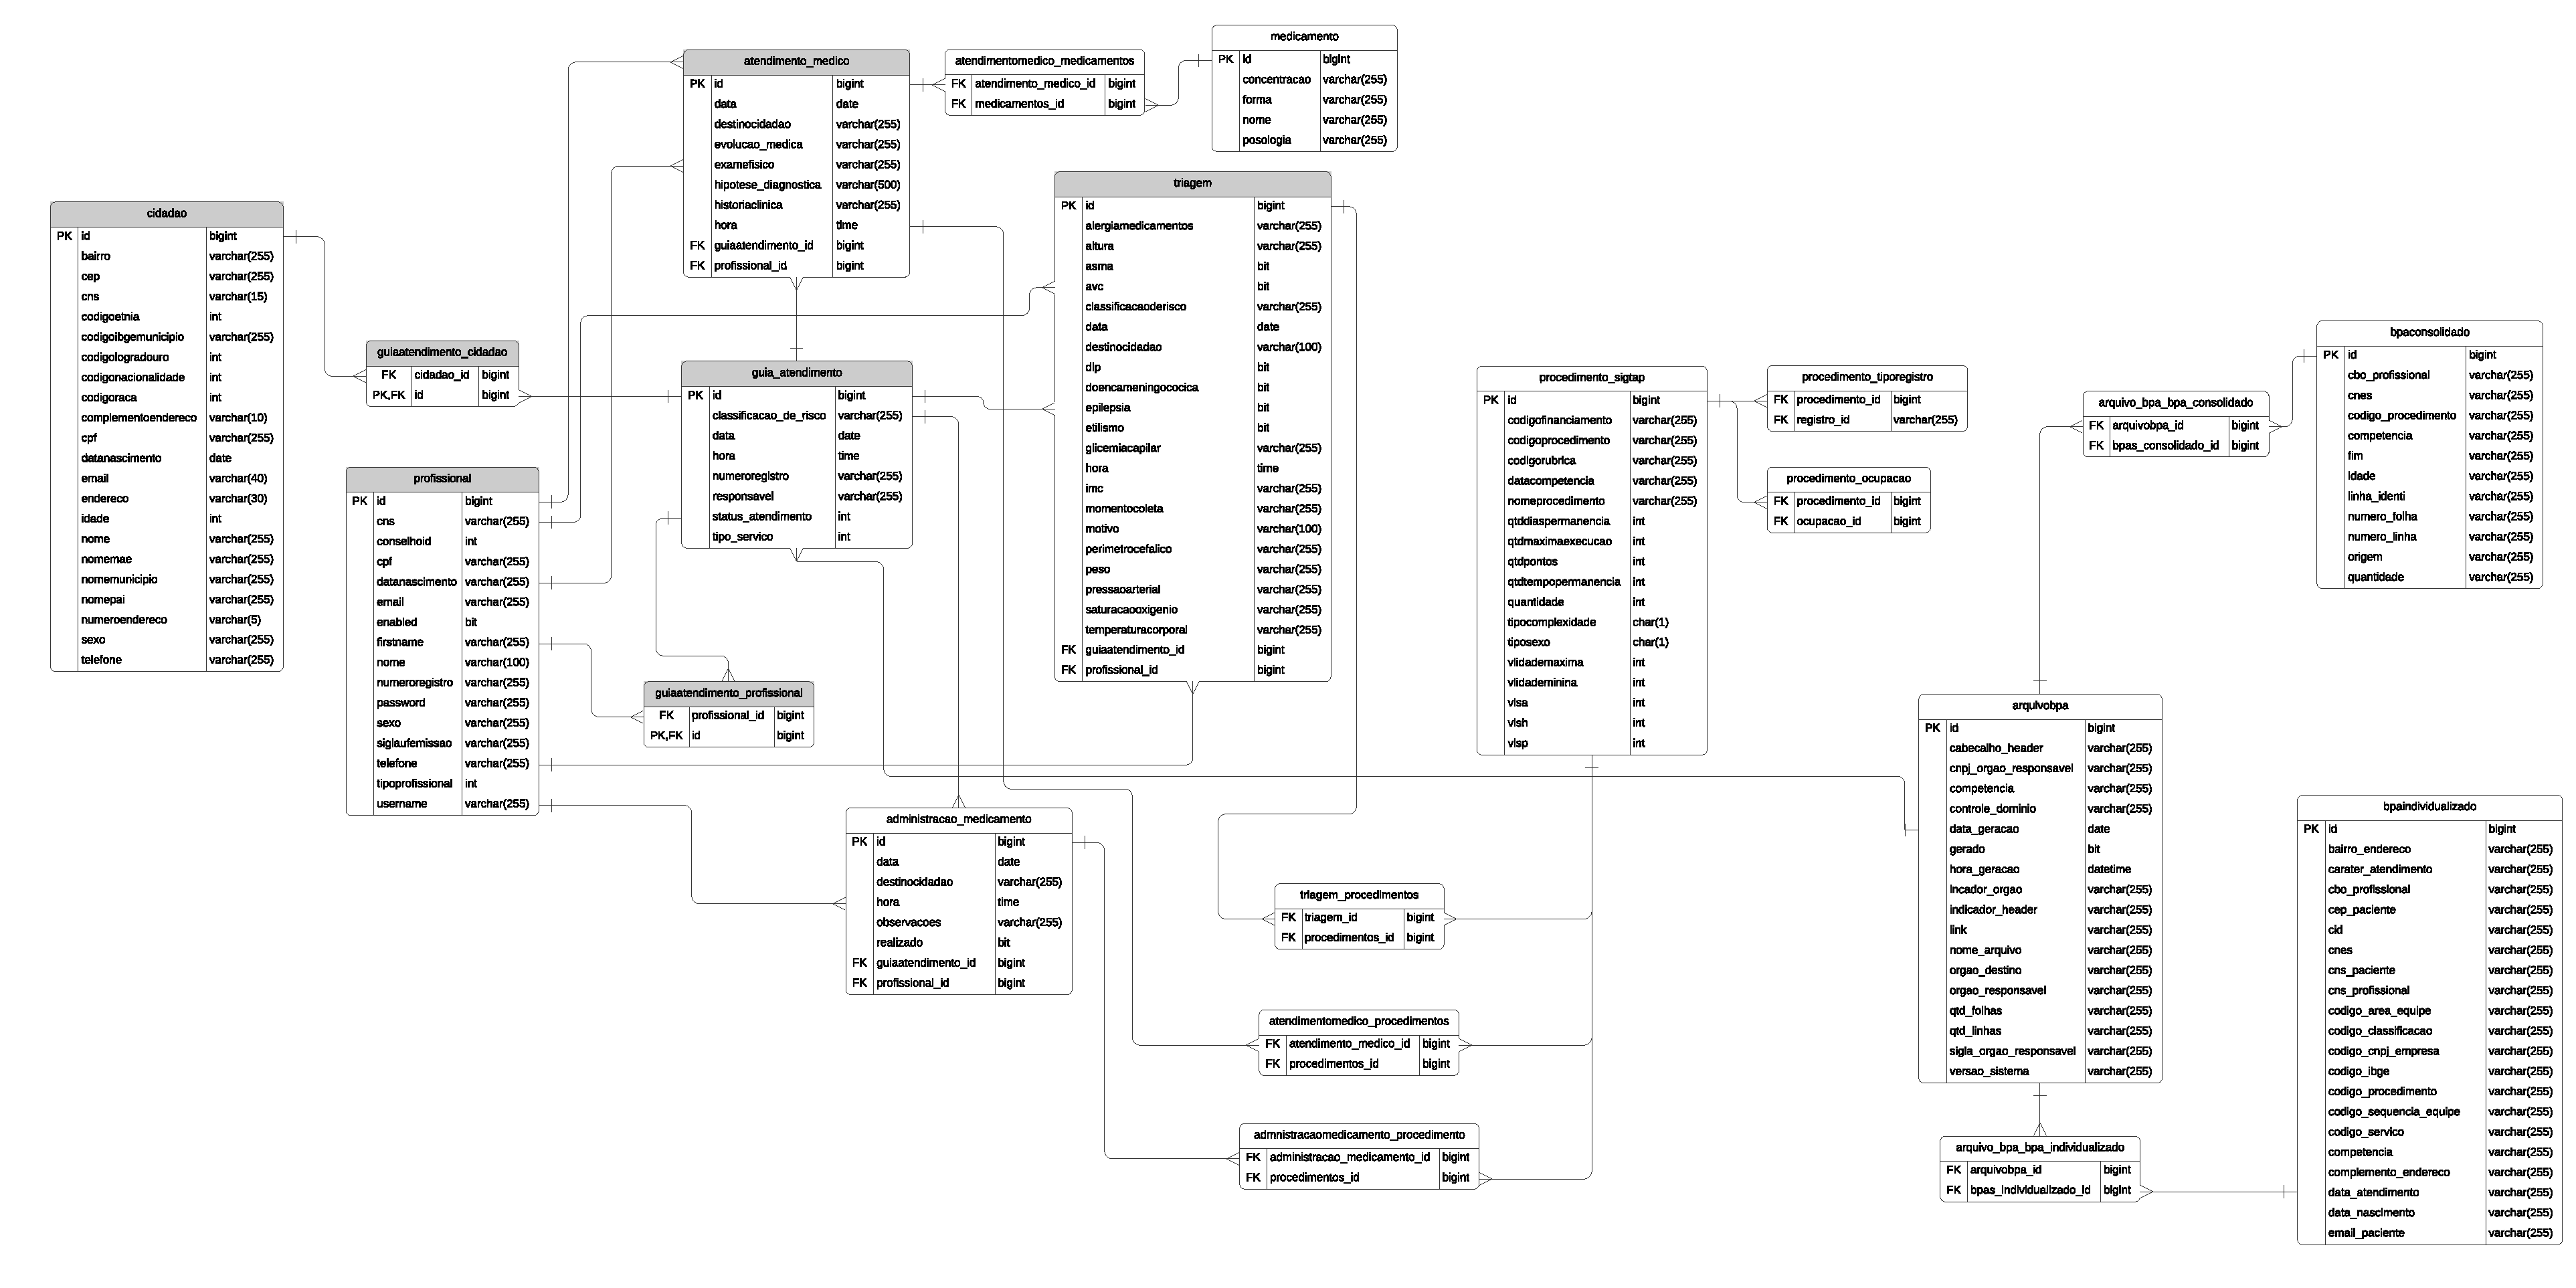
\includepdf[scale=0.75,pages=1,pagecommand=\label{apendice01}\chapter{Diagrama Lógico Banco de Dados}]{apendices/DIAGRAMA-LOGICOBDSGH.pdf}

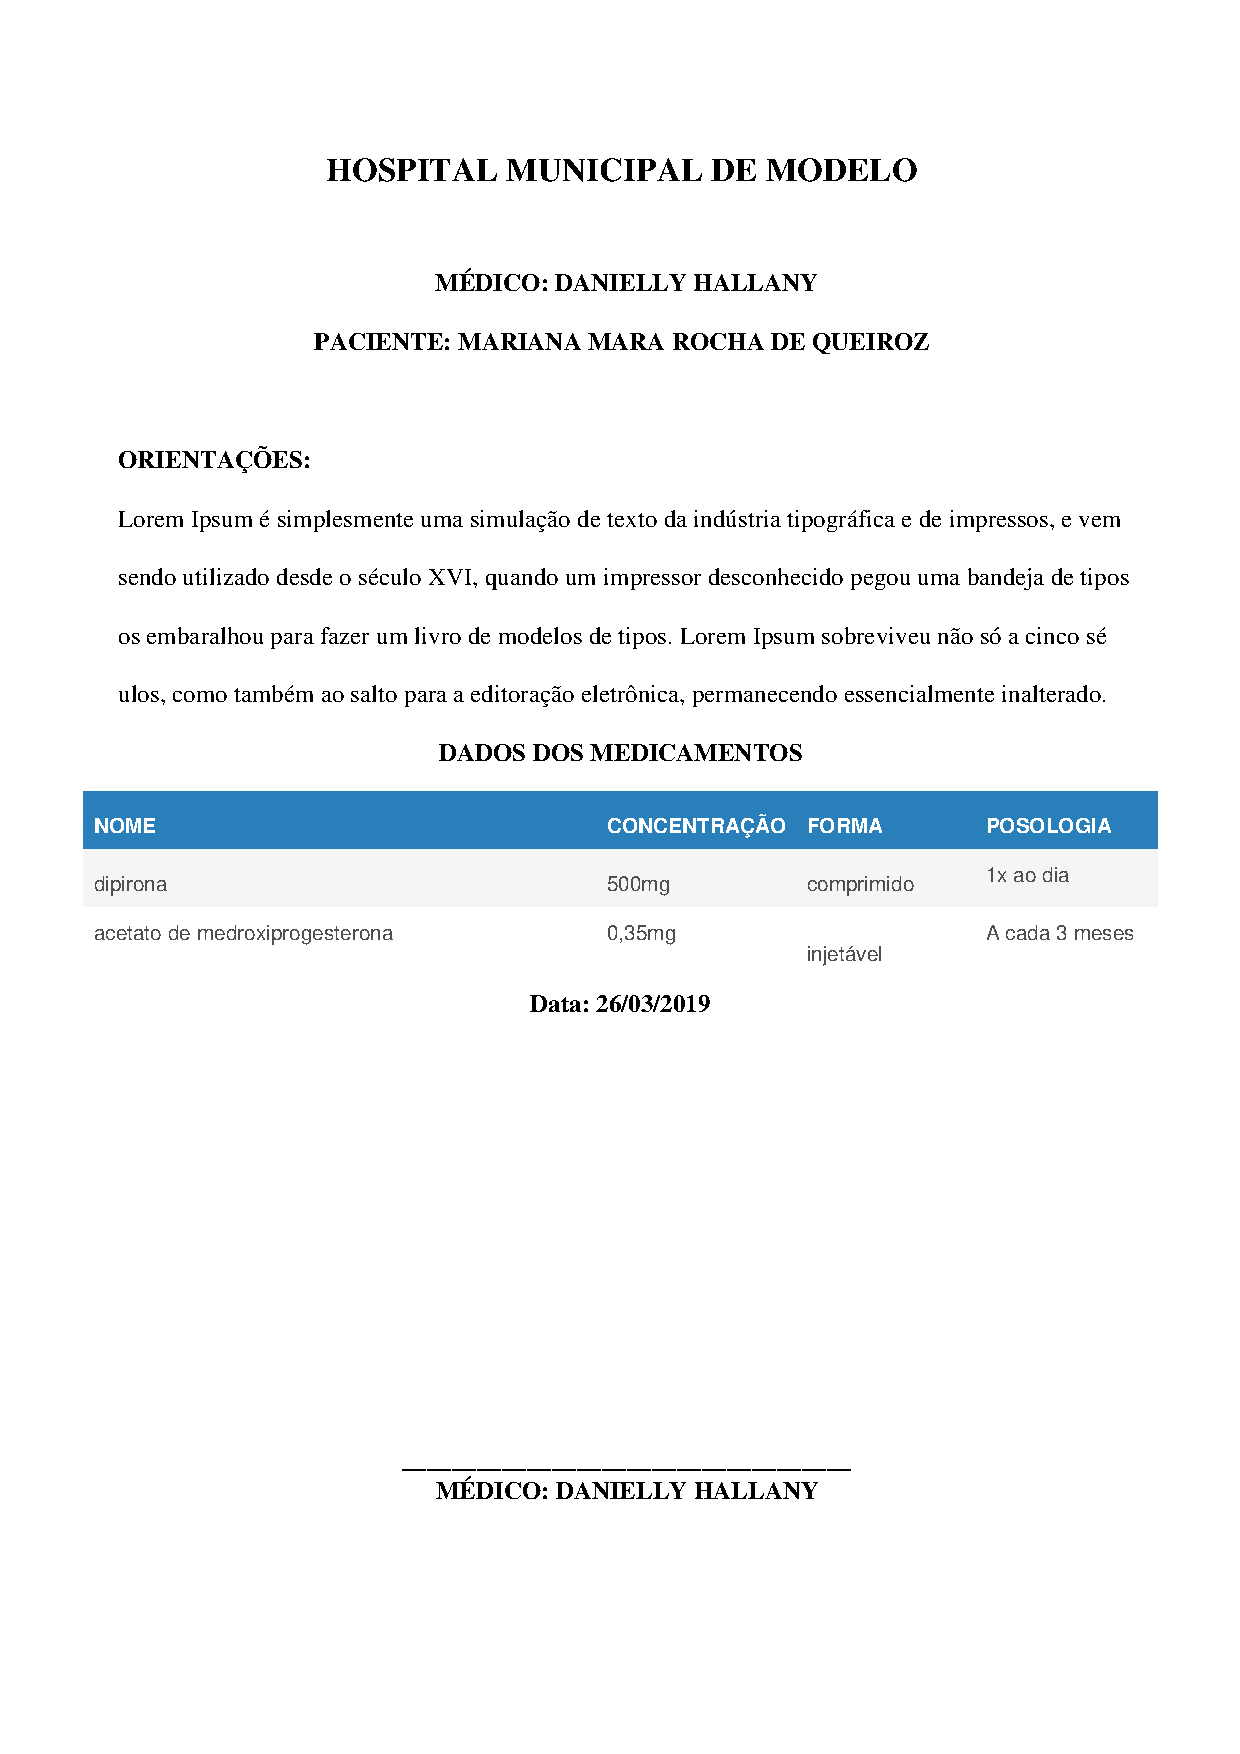
\includepdf[scale=0.75,pages=1,pagecommand=\label{apendice02}\chapter{Impressão do Receituário}]{apendices/Receituario_SGH.pdf}

\end{apendices}

\begin{anexos}
\chapter{Layout da interface texto do BPA e do SIA - Layout INTERNO}
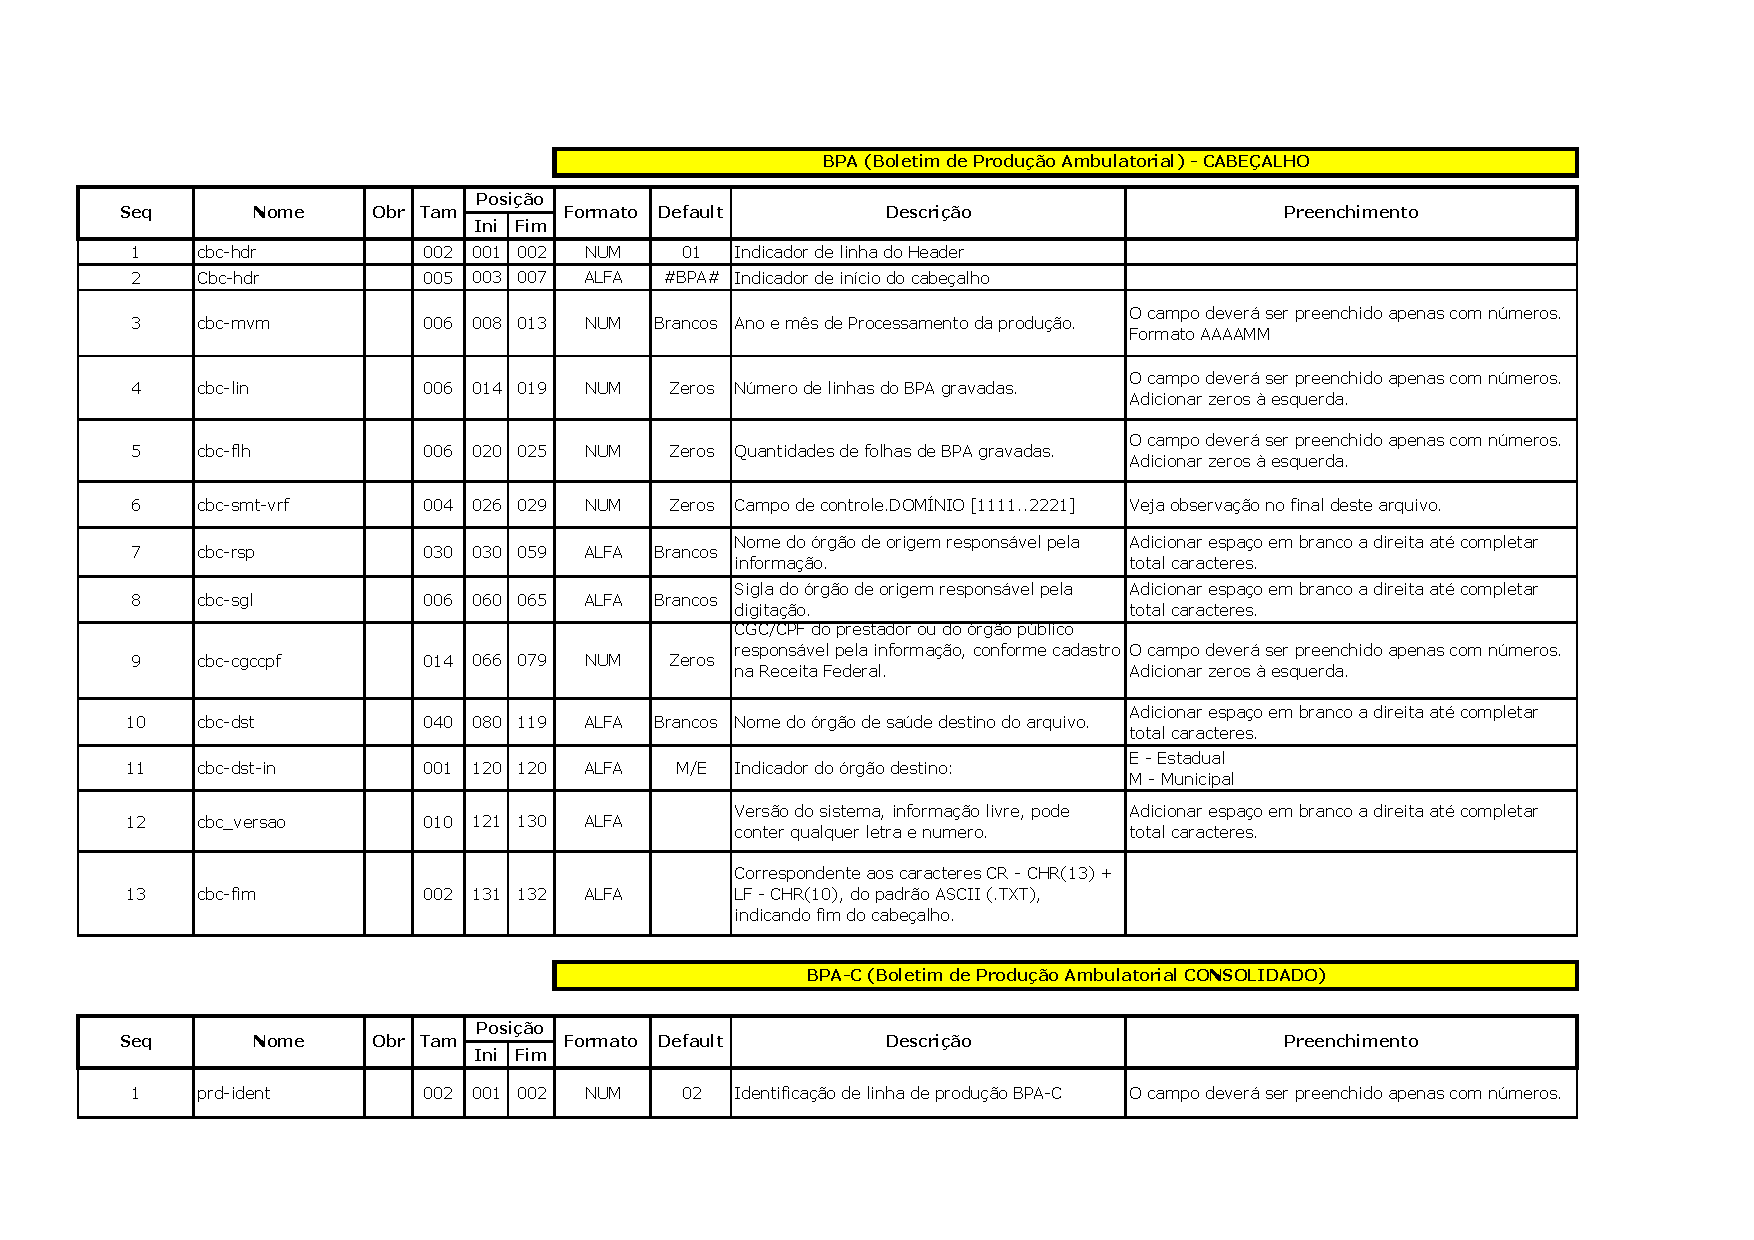
\includepdf[scale=0.95,pages={1-5},landscape]{anexos/Layout_Exportacao_BPA.pdf}
\end{anexos}
\printindex
\end{document}
